%% main.tex modelo de TCC para FEELT-UFU
%% Copyright 2012-2014 by abnTeX2 group at http://abntex2.googlecode.com/ 
%%
%% This work may be distributed and/or modified under the
%% conditions of the LaTeX Project Public License, either version 1.3
%% of this license or (at your option) any later version.
%% The latest version of this license is in
%%   http://www.latex-project.org/lppl.txt
%% and version 1.3 or later is part of all distributions of LaTeX
%% version 2005/12/01 or later.
%%
%% This work has the LPPL maintenance status `maintained'.
%% 
%% The Current Maintainer of this work is the abnTeX2 team, led
%% by Lauro César Araujo. Further information are available on 
%% http://abntex2.googlecode.com/
%%
%% This work consists of the files abntex2-modelo-trabalho-academico.tex,
%% abntex2-modelo-include-comandos and abntex2-modelo-references.bib
%%

% ------------------------------------------------------------------------
% ------------------------------------------------------------------------
% abnTeX2: Modelo de Trabalho Academico (tese de doutorado, dissertacao de
% mestrado e trabalhos monograficos em geral) em conformidade com 
% ABNT NBR 14724:2011: Informacao e documentacao - Trabalhos academicos -
% Apresentacao
% ------------------------------------------------------------------------
% ------------------------------------------------------------------------

\documentclass[
	% -- opções da classe memoir --
	12pt,				% tamanho da fonte
	openright,			% capítulos começam em pág ímpar (insere página vazia caso preciso)
	oneside,			% para impressão em verso e anverso. Oposto a oneside
	a4paper,			% tamanho do papel. 
	% -- opções da classe abntex2 --
	chapter=TITLE,		% títulos de capítulos convertidos em letras maiúsculas
	%section=TITLE,		% títulos de seções convertidos em letras maiúsculas
	%subsection=TITLE,	% títulos de subseções convertidos em letras maiúsculas
	%subsubsection=TITLE,% títulos de subsubseções convertidos em letras maiúsculas
	% -- opções do pacote babel --
	english,			% idioma adicional para hifenização
	french,				% idioma adicional para hifenização
	spanish,			% idioma adicional para hifenização
	brazil				% o último idioma é o principal do documento
	]{abntex2}

% ---
% Pacotes básicos 
% ---
\usepackage{helvet}			% Usa a fonte Latin Modern			
\usepackage[T1]{fontenc}		% Selecao de codigos de fonte.
\usepackage[utf8]{inputenc}		% Codificacao do documento (conversão automática dos acentos)


\usepackage{listings}


\usepackage{lastpage}			% Usado pela Ficha catalográfica
\usepackage{indentfirst}		% Indenta o primeiro parágrafo de cada seção.
\usepackage{color}				% Controle das cores
\usepackage{graphicx}			% Inclusão de gráficos
\usepackage{microtype} 			% para melhorias de justificação
\usepackage{mathtools}
\usepackage{amssymb}
\usepackage{float}


% Desenho de diagramas
\usepackage{tikz}
\usetikzlibrary{shapes,arrows}

% Códigos-fonte


\newsubfloat{figure}% Allow subfloats in figure environment

% ---

% ---
% Pacotes de citações
% ---
\usepackage[brazilian,hyperpageref]{backref}	 % Paginas com as citações na bibl
\usepackage[alf]{abntex2cite}	% Citações padrão ABNT

% --- 
% CONFIGURAÇÕES DE PACOTES
% ---

% Dados gerais do trabalho
\titulo{AMBIENTE SIMULADO PARA CONTROLE DE CALDEIRAS}
\autor{CAIO AUGUSTO ARAÚJO OLIVEIRA}
\local{Uberlândia}
\data{2015}
\orientador{Josué Silva de Morais}
\instituicao{%
  Universidade Federal de Uberlândia
  \par
  Faculdade de Engenharia Elétrica}
\tipotrabalho{Trabalho de Conclusão de Curso}
% O preambulo deve conter o tipo do trabalho, o objetivo, 
% o nome da instituição e a área de concentração 
\preambulo{Trabalho apresentado como requisito parcial de avaliação na disciplina Trabalho de Conclusão de Curso 2 do Curso de Engenharia Elétrica da Universidade Federal de Uberlândia.}




% Relativos ao documento
%% Redefinições do modelo da ABNT/padrões do abntex2.
%
%% ==================================================================
%% ==================================================================
%% NÃO EDITAR ESSE ARQUIVO
%% ==================================================================
%% ==================================================================
%


\renewcommand{\familydefault}{\sfdefault}
\renewcommand{\ABNTEXchapterfontsize}{\bfseries\fontsize{12pt}{1em}}
\renewcommand{\ABNTEXsectionfontsize}{\bfseries\fontsize{12pt}{1em}}
\renewcommand{\ABNTEXsubsectionfontsize}{\bfseries\fontsize{12pt}{1em}}
\renewcommand{\ABNTEXsubsubsectionfontsize}{\bfseries\fontsize{12pt}{1em}}
\renewcommand{\normalsize}{\fontsize{12pt}{1em}}
\renewcommand{\arraystretch}{1.2}

\renewcommand{\legend}{\fontsize{11pt}{1em}}


% Secao Primaria (Chapter): Caixa alta, Negrito, tamanho 12
\makeatletter
\settocpreprocessor{chapter}{%
\let\tempf@rtoc\f@rtoc%
\def\f@rtoc{%
\texorpdfstring{\bfseries\MakeTextUppercase{\tempf@rtoc}}{\tempf@rtoc}}%
}
\makeatother

% Margens
\setlrmarginsandblock{3cm}{2cm}{*} % externa / interna
\setulmarginsandblock{3cm}{2cm}{*} % superior / inferior
\checkandfixthelayout%

% Recuo do paragrafo
\setlength{\parindent}{1.25cm} % normativo citatanto o valor de 1,25 qto 1,5cm
% sem espaco entre os paragrafos
\setlength{\parskip}{0cm}

% Espacamentos nos titulos:
% chapter
\setlength{\beforechapskip}{-\onelineskip} %com 0 nao funcionou
\setlength{\afterchapskip}{\onelineskip} % antes do titulo de capitulo
%\setlength\beforechapskip{-18pt}

% section
\setbeforesecskip{\onelineskip}
\setaftersecskip{\onelineskip}

% subsection
\setbeforesubsecskip{\onelineskip}
\setaftersubsecskip{\onelineskip}

% subsubsection
\setbeforesubsubsecskip{\onelineskip}
\setaftersubsubsecskip{\onelineskip}

% subsubsubsection
\setbeforeparaskip{\onelineskip}
\setafterparaskip{\onelineskip}

% espaçamento duplo
\linespread{2}



% ---
% Configurações do pacote backref
% Usado sem a opção hyperpageref de backref
\renewcommand{\backrefpagesname}{Citado na(s) página(s):~}
% Texto padrão antes do número das páginas
\renewcommand{\backref}{}
% Define os textos da citação
\renewcommand*{\backrefalt}[4]{ }
% 	\ifcase #1 %
% 		Nenhuma citação no texto.%
% 	\or
% 		Citado na página #2.%
% 	\else
% 		Citado #1 vezes nas páginas #2.%
% 	\fi}%
% ---

\renewcommand*{\imprimircapa}{
  \begin{capa}
    \center
    
\includegraphics[width=.62in]{img/template/logo.png}
    
    \ABNTEXchapterfont Universidade Federal de Uberlândia

    \ABNTEXchapterfont Faculdade de Engenharia Elétrica

    \vfill
    
    {\ABNTEXchapterfont\fontsize{16pt}{1em}\textbf{\imprimirautor}}

    \vfill
    {\ABNTEXchapterfont\fontsize{14pt}{1em}\textbf{\imprimirtitulo}}
    \vfill
    \vspace*{1cm}

    \ABNTEXchapterfont\imprimirlocal%
    
    \ABNTEXchapterfont\imprimirdata%
  \end{capa}
}

\renewcommand{\folhaderostocontent}{
  \begin{center}
    
    \vspace*{4.5cm}
    
    {\ABNTEXchapterfont\fontsize{16pt}{1em}\textbf{\imprimirautor}}

    \vfill
    {\ABNTEXchapterfont\fontsize{14pt}{1em}\textbf{\imprimirtitulo}}
    
    \hspace{.45\textwidth}
    \begin{minipage}{.5\textwidth}
    \SingleSpacing%
    \ABNTEXchapterfont\imprimirpreambulo%

    \vspace*{.5cm}
    Orientador: \imprimirorientador%

    \assinatura{Assinatura do Orientador}
    \end{minipage}%
    \vfill 
    
    \ABNTEXchapterfont\imprimirlocal%
    
    \ABNTEXchapterfont\imprimirdata%

  \end{center}
  
}


% Desenho de duagramas de blocos para sistemas de controle
\tikzstyle{block} = [draw, rectangle, 
    minimum height=3em, minimum width=6em]
\tikzstyle{sum} = [draw, circle, node distance=1cm]
\tikzstyle{input} = [coordinate]
\tikzstyle{output} = [coordinate]
\tikzstyle{pinstyle} = [pin edge={to-,thin,black}]



% Estilos de codigos fonte
\newcommand{\Py}[1]{
  \lstinputlisting[
	inputencoding=latin1,
	language=Python,                % choose the language of the code
	basicstyle=\footnotesize,       % the size of the fonts that are used for the code
	% numbers=left,                   % where to put the line-numbers
	% numberstyle=\footnotesize,      % the size of the fonts that are used for the line-numbers
	% stepnumber=1,                   % the step between two line-numbers. If it is 1 each line will be numbered
	% numbersep=5pt,                  % how far the line-numbers are from the code
	backgroundcolor=\color{white},  % choose the background color. You must add \usepackage{color}
	showspaces=false,               % show spaces adding particular underscores
	showstringspaces=false,         % underline spaces within strings
	showtabs=false,                 % show tabs within strings adding particular underscores
	frame=single,           % adds a frame around the code
	tabsize=4,          % sets default tabsize to 2 spaces
	captionpos=b,           % sets the caption-position to bottom
	breaklines=true,        % sets automatic line breaking
	breakatwhitespace=false,    % sets if automatic breaks should only happen at whitespace
        mathescape=false,
        texcl=false
%	escapeinside={\%*}{*)},          % if you want to add a comment within your code
  ]{\detokenize{srcs/py/#1.py}}
}


% ---
% Configurações de aparência do PDF final

% alterando o aspecto da cor azul
\definecolor{blue}{RGB}{41,5,195}

% informações do PDF
\makeatletter
\hypersetup{
     	%pagebackref=true,
		pdftitle={\@title}, 
		pdfauthor={\@author},
    	        pdfsubject={\imprimirpreambulo},
	        pdfcreator={LaTeX with abnTeX2},
		pdfkeywords={abnt}{latex}{abntex}{abntex2}{trabalho acadêmico}, 
		colorlinks=true,       		% false: boxed links; true: colored links
    	        linkcolor=blue,          	% color of internal links
    	        citecolor=blue,        		% color of links to bibliography
    	        filecolor=magenta,      		% color of file links
		urlcolor=blue,
		bookmarksdepth=4
}
\makeatother
% --- 

% --- 
% Espaçamentos entre linhas e parágrafos 
% --- 

% O tamanho do parágrafo é dado por:
\setlength{\parindent}{1.3cm}

% Controle do espaçamento entre um parágrafo e outro:
\setlength{\parskip}{0.2cm}  % tente também \onelineskip



% ---
% compila o indice
% ---
\makeindex
% ---

% ----
% Início do documento
% ----
\begin{document}

% Retira espaço extra obsoleto entre as frases.
\frenchspacing 

% ---
% Capa
% ---
\imprimircapa%
% ---

% ---
% Folha de rosto
% (o * indica que haverá a ficha bibliográfica)
% ---
\imprimirfolhaderosto%
% ---

% % ---
% % Dedicatória
% % ---
% \begin{dedicatoria}
%    \vspace*{\fill}
%    \centering
%    \noindent
%    \textit{ Dedico esse trabalho à minha família, pela paciência e compreensão.
 } \vspace*{\fill}
% \end{dedicatoria}
% ---

% ---
% Agradecimentos
% ---
\begin{agradecimentos}
  Ao Professor Josué Silva de Morais pelo incentivo, motivação e
orientação deste trabalho.

Ao Laboratório de Automação, Servomecanismos e Controle da Faculdade
de Engenharia Elétrica da Universidade Federal de Uberlândia, pela
ajuda e pela infraestrutura de qualidade disponibilizada para o
desenvolvimento deste trabalho.

À minha família e amigos, pelo apoio, paciência e incentivos durante
todo o meu período acadêmico.

À minha namorada, Thaís, pelo suporte, carinho e ajuda em todas as
fases da minha formação.

Em especial aos meus pais, pela dedicação, comprometimento, paciência
e por serem o modelo de ser humano que tento seguir.

\end{agradecimentos}
% ---

% ---
% RESUMOS
% ---

% resumo em português
\setlength{\absparsep}{18pt} % ajusta o espaçamento dos parágrafos do resumo
\begin{resumo}
  Esse trabalho apresenta a construção de um simulador das propriedades
dinâmicas de uma caldeira de vapor aquatubular. O objetivo é
disponibilizar uma forma confiável e segura de se trabalhar com um
sistema similar ao de uma caldeira em funcionamento, utilizando um
modelo matemático dinâmico não linear para a representação das
propriedades da caldeira com relação a variações em parâmetros como
pressão, vazões de água e vapor e fluxo de calor. Também é apresentada
a forma de comunicação com o simulador, de forma que seja simples
construir novas aplicações que se integrem ao mesmo e possibilitando
também a construção de drivers para comunicação com outros
equipamentos. Para atestar o funcionamento correto do simulador, uma
interface gráfica, um controlador de nível de água e um controlador de
pressão serão desenvolvidos.

\end{resumo}

% resumo em inglês
\begin{resumo}[Abstract]
  This work presents the construction of a dynamic water-tube boiler
simulator. The goal is to develop a reliable and safe way to work with
a system that is similar to the working boiler, using a non linear
dynamic mathematical model to represent the boiler's properties with
relation to variations in several parameters, like pressure and water
and heat flows. It is also presented a way of communicating with the
simulator, in a way that is simple to build new applications to
integrate with it, allowing the development of new drivers for
communicating with other equipments. To ensure the correct functioning
of the simulator, an interface app, a pressure controller and water
level controller will be built.

\end{resumo}

% ---
% inserir lista de ilustrações
% ---
\pdfbookmark[0]{\listfigurename}{lof}
\listoffigures*
\cleardoublepage
% ---

% ---
% inserir lista de tabelas
% ---
\pdfbookmark[0]{\listtablename}{lot}
\listoftables*
\cleardoublepage
% ---

% ---
% inserir lista de abreviaturas e siglas
% ---
\begin{siglas}
  \item[CLP] Controlador lógico programável
\item[PWR] Reator de água pressurizada
\item[LT] Transmissor de nível
\item[FT] Transmissor de vazão
\item[LRC] Controlador de nível
\item[FY] Dispositivo de cálculo
\item[FIC] Controlador de vazão
\item[PID] Controlador proporcional, integral e derivativo
\item[TCP] Transmission Control Protocol
\item[IP] Internet Protocol
\item[POSIX] Portable operating system interface
\item[MQ] Sistema de fila de mensagens
\item[FIFO] First-in-first-out
\item[PI] Controle proporcional integral

\end{siglas}
% ---

% ---
% inserir lista de símbolos
% ---
\begin{simbolos}
    \item[$ q_f $] Vazão mássica de água entrando na caldeira
  \item[$ q_s $] Vazão mássica de saída de vapor da caldeira
  \item[$ q_{ct} $] Vazão mássica de condensação de água
  \item[$ q_{dc} $] Vazão mássica entrando no tubo ascendente
  \item[$ q_r $] Vazão mássica saindo do tubo ascendente
  \item[$ q_{sd} $] Vazão mássica de vapor através da superfície do
  líquido
  \item[$ q_{cd} $] Vazão mássica de condensação no tubulão
  \item[$ q_{ct} $] Vazão mássica de condensação na caldeira

  \item[$ V_{wt} $] Volume total de água
  \item[$ V_{st} $] Volume total de vapor
  \item[$ V_r $] Volume do interior do tubo ascendente
  \item[$ V_t $] Volume total da caldeira
  \item[$ V_{wd} $] Volume de água líquida abaixo do nível de líquido
  \item[$ V_{sd} $] Volume de vapor abaixo do nível de líquido
  \item[$ V_{sd}^0 $] Valor de $V_{sd}$ para situação hipotética em
  que não há condensação do vapor no interior da caldeira
  \item[$ V_d $] Volume do tubulão

  \item[$ \rho_s $] Densidade do vapor
  \item[$ \rho_w $] Densidade da água
  
  \item[$ u_s $] Energia interna do vapor
  \item[$ u_w $] Energia interna da água
  
  \item[$ h_f $] Entalpia da água de alimentação
  \item[$ h_s $] Entalpia do vapor
  \item[$ h_w $] Entalpia da água da caldeira
  \item[$ h_c $] Entalpia de condensação

  \item[$ \alpha_m $] Fração que consiste de vapor da vazão mássica no
  tubo ascendente
  \item[$ \alpha_v $] Fração volumétrica de vapor
  \item[$ \alpha_r $] Qualidade do vapor que sai do tubo ascendente
  \item[$ \bar{\alpha_v} $] Fração volumétrica média de vapor

  \item[$ l $] Variação do nível de água no tubulão superior, medida a
  partir do ponto de operação normal
  \item[$ l_w $] Contribuição do líquido na variaçao do nível de água
  no tubulão
  \item[$ l_s $] Contribuição do vapor na variaçao do nível de água no
  tubulão

  \item[$ l_o $] Variação do nível de água no tubulão superior, medida
  a partir do ponto de operação normal
  \item[$ l_{wo} $] Contribuição do líquido na variaçao do nível de
  água no tubulão
  \item[$ l_{so} $] Contribuição do vapor na variaçao do nível de água
  no tubulão


  \item[$ L_r $] Comprimento do tubo ascendente
  \item[$ L_{dc} $] Comprimento do tubo descendente

  \item[$ A_{dc} $] Área da seção transversal do tubo
  descendente \item[$ A_d $] Superfície molhada quando o nível se
  encontra em seu ponto de operação

  \item[$ k $] Coeficiente de fricção nos tubos

  \item[$ \xi $] Comprimento normalizado do tubo ascendente, com
  relação ao eixo $Z$

  \item[$ p $] Pressão da caldeira
  \item[$ m_t $] Massa total do metal dos tubos
  \item[$ C_p $] Calor específico do metal
  \item[$ t_m $] Temperatura do metal
  \item[$ t_s $] Temperatura de saturação do vapor
  \item[$ Q $] Taxa de fluxo de calor nos tubos ascendentes
  \item[$ g $] Aceleração gravitacional
  \item[$ T_d $] Tempo de permanêncial do vapor no tubulão
  \item[$ \beta $] Constante empírica

  \item[$ X $] Vetor de variáveis de estado
  \item[$ U $] Vetor de variáveis de entrada
  \item[$ E $] Função das variáveis de estado
  \item[$ e_{ij} $] Valor de célula na linha $i$ e coluna $j$ da
  matriz $E$



\end{simbolos}
% ---

% ---
% inserir o sumario
% ---

\pdfbookmark[0]{\contentsname}{toc}

% Nível máximo listado no sumário
\settocdepth{subsubsection}

\tableofcontents*
\cleardoublepage
% ---



% ----------------------------------------------------------
% ELEMENTOS TEXTUAIS
% ----------------------------------------------------------


\textual
\pagestyle{chapter}

% ----------------------------------------------------------
% Introdução (exemplo de capítulo sem numeração, mas presente no Sumário)
% ----------------------------------------------------------
\chapter[Introdução]{Introdução}

% ----------------------------------------------------------

O uso de caldeiras aquatubulares é amplamente difundido, sendo comum
em plantas termelétricas ou para geração de energia elétrica em geral
\cite{wikicaldeiras}. No Brasil, o aumento do interesse em fontes
alternativas de energia causado pela crise energética de 2001 resultou
em um aumento da utilização de biomassa como forma de diversificação
da matriz energética do país \cite{dantasusp}. Essa utilização causou
o aumento significativo da utilização de caldeiras de geração de vapor
na indústria sucroalcooleira, onde o resíduo da produção de etanol a
partir da cana de açúcar é usado em sistemas de cogeração de energia
elétrica capazes de suprir toda a demanda eletromecânica e térmica das
usinas e destilarias, operando em Ciclo Rankine com turbinas a vapor
de contrapressão \cite{leme2005}.

Estudos mostram que o nível de água na caldeira é uma das variáveis
mais importantes para o funcionamento correto e seguro de uma
caldeira: em 1995, foi constatado que 30\% das paradas emergenciais de
plantas nucleares do tipo PWR (reator de água pressurizada) na França
foram causadas por uma variação do nível de água do
tubulão \apud{kwatny}{astrom}, mostrando que o controle dessa variável
é extremamente importante.

Um nível de água elevado dificulta a separação entre líquido e vapor,
aumentando a umidade contida no vapor e diminuindo sua qualidade,
podendo chegar a danificar as pás da turbina. Já o baixo nível de água
pode fazer com que a água restante evapore rapidamente em operação com
carga elevada. Essa evaporação rápida pode causar o superaquecimento
da caldeira, podendo queimá-la ou resultar em uma
explosão \cite{yuan}. O superaquecimento da caldeira também aumenta a
necessidade de paradas da planta, além de aumentar os riscos à
segurança \cite{habib}.

O desenvolvimento de sistemas de controle de nível em caldeiras
aquatubulares já foi amplamente estudado, como pode ser visto
em \citeonline{ufrj} e \citeonline{yuan}.  A simulação de uma caldeira
também já foi exaustivamente discutida em outros trabalhos,
como \citeonline{astrom}, \citeonline{adam1999} e \citeonline{habib},
com resultados próximos aos reais \cite{astrom}, porém especificações
detalhadas para implementação de um simulador não estão disponíveis
nesses trabalhos, o que dificulta a utilização prática dos resultados
encontrados.

A partir de modelos dinâmicos do comportamento do nível da caldeira, é
possível projetar um sistema de controle de nível e validá-lo através
do teste em simuladores, como feito em \citeonline{ufrj}. Após o
projeto, um CLP deve ser programado com a lógica desenvolvida e então
inserido na planta. Um possível defeito no CLP só será constatado
durante sua implantação, quando a planta (ou parte dela) está
desligada. Nesses casos, encontrar o problema com o CLP pode ser mais
difícil, pois o técnico estará sob estresse \cite{troubleshootplc},
além de atrasar o reinicio da planta e portanto gerar prejuízos.

Esse trabalho tem como objetivo a implementação de um simulador do
comportamento dinâmico de uma caldeira aquatubular. Espera-se produzir
um sistema de simulação versátil e de fácil configuração. Esse sistema
deverá ter uma interface de comunicação simples, possibilitando a
criação de drivers para diferentes tipos de controladores e sistemas
supervisórios.



\chapter[Desenvolvimento]{Desenvolvimento}

\section{Revisão Bibliográfica}
% Revisão bibliográfica
%
% Fundamentação teórica do trabalho. Aqui deve ser revisto tudo o que
% foi utilizado para a concepção do trabalho.

\subsection{Caldeiras aquatubulates}

\begin{figure}[H]
\caption{\label{fig_circulo} Esquema de uma caldeira aquatubular}
\begin{center}
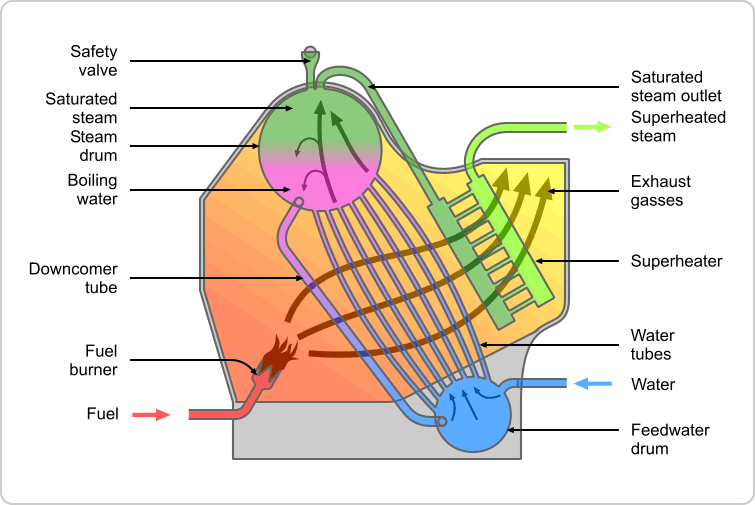
\includegraphics[scale=0.75]{img/caldeira.png}
\end{center}
\legend{Fonte: \citeonline{wikiwatertube}}
\end{figure}

O que diferencia uma caldeira aquatubular das outras é a localização
da água e do sistema de combustão: a água fica dentro de tubos,
enquanto a combustão ocorre fora dos tubos. Também pode-se dizer que o
material dos tubos sofre forças de tensão, uma vez que a pressão é
gerada internamente \cite{boilers}. Um esquema simplificado da
caldeira pode ser visto na figura \ref{fig_circulo}.

\subsubsection{Funcionamento}
Na caldeira aquatubular, existem dois tubulões ligados por dois
conjuntos de tubos: ascendentes e descendentes. Um dos tubulões fica
em baixo, alimentado por uma entrada de água. O tubulão superior é
preenchido até um certo nível por água, sendo o restante preenchido
por vapor. No tubulão superior o vapor é coletado, normalmente
passando por um superaquecedor para diminuir a umidade do vapor que
alimentará a planta.

O calor é transferido para a água através dos tubos ascendentes. Por
causa do aquecimento direto dos tubos, uma diferença entre a densidade
da água no tubo ascendente e o tubo descendente faz com que ocorra uma
circulação de água natural entre os tubos. Dessa forma, a água
aquecida sobe pelos tubos ascendentes, libera o vapor no tubulão
superior e então retorna para o tubulão inferior através dos tubos
descendentes \cite{ufrj}. Para caldeiras de maior pressão, as
densidades da água nos tubos ascendentes e descendentes começam a
assumir valores próximos, impossibilitando a circulação natural da
água. Nessas caldeiras, bombas hidráulicas são acionadas e circulam a
água na caldeira.

Para se controlar o nível do tubulão, atua-se na válvula de entrada de
água, ou seja, alterando a vazão de entrada de água. A
diferença entre a vazão de entrada e a vazão de saída (na forma de
vapor) proporciona o aumento ou diminuição do nível de água no tubulão
superior, ao alterar a quantidade total de água no sistema. Isso pode
ser visto na equação a seguir:


\begin{equation}
  \dfrac{d}{dt} (\rho_s V_{st} + \rho_w V_{wt}) = q_f - q_s
  \label{balanco_global_massa}
\end{equation}

Aqui, os subscritos $s$ e $w$ se referem ao vapor e água,
respectivamente. $\rho$ e $q$ são, respectivamente, densidades
e vazões mássicas. $V_{st}$ e $V_{wt}$ são os volumes de vapor e água
dentro da caldeira.


Esse volume total de água influencia diretamente o nível de água no
tubulão, porém não é a única variável. Efeitos de dilatação e
contração devidos à mudanças na pressão e na temperatura também
influenciam o nível, o que faz o controle do mesmo ser uma tarefa
complicada \cite{astrom}. Em \citeonline{astrom} é desenvolvido um
modelo matemático dinâmico com o intuito de representar essa variação
do nível em caldeiras de grande porte e circulação natural de
água. A construção desse modelo é apresentada a seguir.

\subsection{Modelo matemático}

A maior parte do comportamento dinâmico do sistema pode ser descrito
através dos balanços de massa e energia globais do sistema. A equação
\ref{balanco_global_massa} é o balanço global de massa, enquanto a equação do
balanço global de energia pode ser escrita como:

\begin{equation}
  \dfrac{d}{dt} (\rho_s u_s V_{st} + \rho_w u_w V_{wt} + m_t C_p t_m)
  = Q + q_f h_f - q_s h_s
  \label{balanco_global_energia0}
\end{equation}

O lado direito da equação \ref{balanco_global_energia0} mostra o fluxo
de energia que é recebido através do calor proveniente da queima do
combustível, somado à energia interna da água de alimentação ($ Q +
q_f h_f $). Também mostra o fluxo de energia entregue pela caldeira
através do vapor ($q_s h_s$).

Onde $h$ é entalpia, $u$ é energia interna, $m_t$ é a massa total de
metal dos tubos, $C_p$ é o calor específico do metal e $t_m$ é a
temperatura do mesmo. \citeonline{astrom} diz que o sistema pode ser
considerado sempre termicamente em equilíbrio, ou seja, considera-se a
temperatura do metal igual à temperatura de saturação do vapor
($t_s$), que é função da pressão $p$ da caldeira.

A equação a seguir relaciona os volumes de água e vapor com o volume
total da caldeira ($V_t$):
\begin{equation}
  V_t=V_{wt}+V_{st}
  \label{vol_total}
\end{equation}

A energia interna de um sistema pode ser representada como $u = h - p
/ \rho$, onde $p$ é a pressão interna da caldeira. Utilizando a
equação \ref{vol_total} e a relação da energia interna, pode-se
reescrever a equação \ref{balanco_global_energia0} da seguinte forma:

\begin{equation}
  \dfrac{d}{dt} (\rho_s h_s V_{st} + \rho_w h_w V_{wt} - p V_t + m_t C_p t_m)
  = Q + q_f h_f - q_s h_s
  \label{balanco_global_energia}
\end{equation}

Em uma caldeira, as variáveis $Q$, $q_f$ e $q_s$ podem ser mensuradas
direta ou indiretamente. $q_s$ depende da demanda da planta, enquanto
$Q$ é controlado por malhas externas ao controle de nível. A variável
$q_f$ é usada como variável de controle, uma vez que o sistema atua na
válvula de entrada de água para o controle de nível. A saída do
sistema será sua pressão ($p$) e o nível da água no tubulão superior
($l$).

$\rho_w$, $\rho_s$, $h_w$, $h_s$, e $t_s$ são propriedades
térmodinâmicas da água. Por estarem a temperatura próxima da
temperatura de saturação, pode-se representá-las como função somente
da pressão \cite{garland}. Já as propriedades termodinâmicas da água
de alimentação, por esta estar a uma baixa temperatura em relação ao
sistema, podem ser consideradas funções somente da temperatura
\cite{garland2}.

Por enquanto as equações \ref{balanco_global_massa} e
\ref{balanco_global_energia} conseguem descrever o comportamento da
pressão e da quantidade de água total com relação a alterações no
calor e vazões de entrada de água e saída de vapor, mas não descreve o
comportamento do nível de água, uma vez que, por serem equações de
balanços globais, não apresentam informações sobre a distribuição do
vapor no interior do tubulão. É a forma de distribuição do vapor e da
água no interior da caldeira que dá origem aos efeitos de contração
e expansão, uma vez que o vapor pode estar localizado abaixo do nível
da água na forma de pequenas bolhas, o que caracteriza um sistema de
escoamento bifásico.

Sistemas de escoamento bifásico são normalmente modelados usando
equações diferenciais parciais e elementos finitos, mas um modelo
simplificado do mesmo é suficiente para a simulação da caldeira.

Esse modelo pode ser encontrado usando os balanços de massa e energia
no tubo ascendente. As equações são, respectivamente:

\begin{equation}
  A\dfrac{\partial \rho} {\partial t} + \dfrac{\partial q}{\partial z}
  = 0
  \label{balanco_massa_riser}
\end{equation}

\begin{equation}
  \dfrac{\partial \rho h}{\partial t} + \dfrac{1}{A} \dfrac{\partial q
    h}{\partial z} = \dfrac{Q}{V}
  \label{balanco_energia_riser}
\end{equation}

No caso, as variáveis são:
\begin{itemize}
\item[$ \rho $]: Densidade da mistura de água e vapor
\item[$ t $]: Tempo
\item[$ q $]: Vazão mássica da mistura
\item[$ h $]: Entalpia da mistura
\item[$ A $]: Área de uma seção transversal
\item[$ V $]: Volume do tubo
\item[$ Q $]: Calor entregue ao tubo
\end{itemize}

\begin{figure}[H]
  \caption{\label{riser} Esquema simplificado das variáveis dinâmicas
    do tubo ascendente}
  \begin{center}
    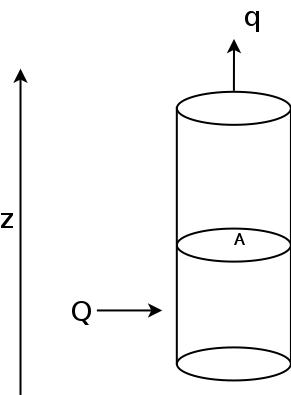
\includegraphics[scale=0.3]{img/riser.png}
  \end{center}
\end{figure}

Para simplificar o modelo, foi considerado que a variação das
variáveis com relação aos eixos $X$ e $Y$ é nula, portanto todas as
variáveis do sistema são funções de $z$ e $t$.

Então, se $\alpha_m$ é definida como a fração do fluxo mássico
constituída de vapor, tem-se a seguinte equação:

\begin{equation}
  h=\alpha_m h_s + (1-\alpha_m) h_w = h_w + \alpha_m h_c
  \label{entalpia_mist_riser}
\end{equation}


Em regime permanente, as seguintes igualdades são derivadas das
equações \ref{balanco_massa_riser} e \ref{balanco_energia_riser}:

\begin{equation}
  \dfrac{\partial q}{\partial z} = 0
  \label{balanco_massa_riser_rp}
\end{equation}

\begin{equation}
  \dfrac{1}{A} \dfrac{\partial q h}{\partial z} = \dfrac{Q}{V}
  \label{balanco_energia_riser_rp}
\end{equation}


Substituindo as equações \ref{balanco_massa_riser_rp} e
\ref{balanco_energia_riser_rp} na equação \ref{entalpia_mist_riser},
tem-se:

\begin{equation}
  \alpha_m = \dfrac{Q A}{q h_c V} z
  \label{eq_alfa_m}
\end{equation}

Para facilitar os cálculos, define-se a variável $\xi$ como o
comprimento normalizado do tubo ascendente, ou seja, se $ L $ é o
comprimento total do tubo e $L_i$ um comprimento qualquer, tem-se
$\xi=L_i / L$. Logo, $0 \leq \xi \leq 1$.

Define-se a qualidade do vapor que sai em um ponto do tubo ascendente 
como $\alpha_r$, relacionando-se com $\alpha_m$ da seguinte maneira:

\begin{equation}
  \alpha_m(\xi)=\alpha_r\xi
  \label{alpha_r_m_lin}
\end{equation}

Na realidade, existe um escorregamento entre o vapor e a água que
causa uma não linearidade na relação entre $\alpha_m$ e $\alpha_r$,
porém de acordo com dados experimentais o escorregamento pode ser
ignorado \cite{astrom}.

A fração volumétrica também é uma função da fração mássica, definida
da seguinte forma:

\begin{equation}
  \alpha_v=\dfrac{ \rho_w \alpha_ m}{ \rho_s + (\rho_w - \rho_s) *
    \alpha_m } 
  \label{alpha_v_alpha_m}
\end{equation}

Essa modelagem, apesar de utilizar o modelo linear para o cálculo de
$\alpha_m$, mostrou-se próxima dos dados reais, como mostra o gráfico
da figura \ref{alpha_v_pde_lin}.

\begin{figure}[H]
  \caption{\label{alpha_v_pde_lin} Comparação entre resultados em
    regime permanente do modelo simplificado de $\alpha_v$ e
    resolução de equações diferenciais parciais}
  \begin{center}
    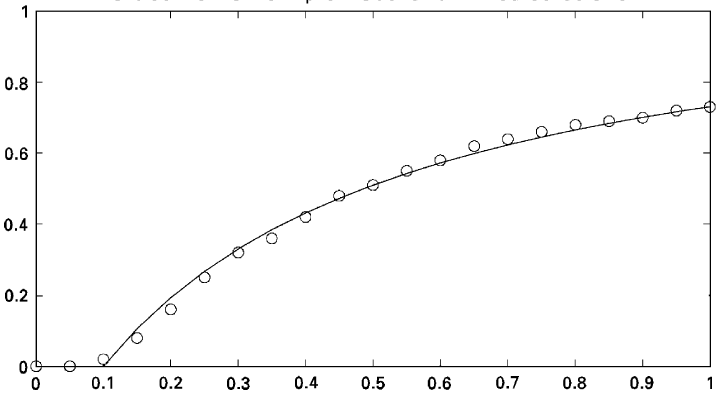
\includegraphics[scale=0.25]{img/alpha_v_pde_lin.png}
  \end{center}
  \legend{Fonte: \cite{astrom}. A linha contínua representa o modelo
    simplificado (equações \ref{alpha_r_m_lin} e
    \ref{alpha_v_alpha_m}), enquanto os círculos representam soluções
    numéricas a partir de equações diferenciais parciais complexas. }
\end{figure}

Para encontrar o nível de água, é necessário encontrar o volume total
de vapor nos tubos ascendentes. Para isso, é necessário encontrar a
fração volumétrica média ($ \bar{\alpha_v} $) nos tubos:

\begin{center}
  $\bar{\alpha}_v = \dfrac{1}{\alpha_m(1)} \int_0^{\alpha_m(1)}
  \alpha_v(\alpha_m) d\alpha_m $
\end{center}

A partir da equação \ref{alpha_r_m_lin}, pode-se perceber que
$\alpha_m(1) = \alpha_r$ e $d\alpha_m = \alpha_r d\xi$. Logo

\begin{center}
  $\bar{\alpha}_v = \dfrac{1}{\alpha_r} \int_0^{\alpha_r}
  \alpha_v(\xi) \alpha_r d\xi$
\end{center}

\begin{equation}
  \bar{\alpha}_v = \dfrac{\rho_w}{\rho_w - \rho_s}
  \biggl( 1 - \dfrac{\rho_s}{(\rho_w - \rho_s)\alpha_r} ln\biggl( 1 +
  \dfrac{\rho_w - \rho_s}{\rho_s} \alpha_r \biggr) \biggr)
  \label{alfa_v_avg}
\end{equation}

Outro elemento importante para a simulação é a transferência de massa
e energia entre o vapor e a água através da condensação e
evaporação. Para evitar a necessidade de contabilizar explicitamente
tal transferência, as equações de balanço energético e mássico da água
e vapor são escritas em conjunto, sendo o balanço global de massa nos
tubos ascendentes representado por

\begin{equation}
  \dfrac{d}{dt} (\rho_s \bar{\alpha}_v V_r + \rho_w (1 -
  \bar{\alpha}_v)V_r) = q_{dc} - q_r
  \label{balanco_massa_riser}
\end{equation}

Onde $q_r$ e $q_{dc}$ são, respectivamente, os fluxos mássicos saindo
e entrando do tubo ascendente.

O balanço global de energia no tubo ascendente é

\begin{equation}
  \dfrac{d}{dt} (\rho_s h_s \bar{\alpha}_v V_r + \rho_w h_w (1 -
  \bar{\alpha}_v)V_r - pV_r + m_r C_p t_s) = Q + q_{dc} h_w -
  (\alpha_r h_c + h_w) q_r
  \label{balanco_energia_riser}
\end{equation}

Onde $h_c$ é a entalpia de condensação:

\begin{equation}
  h_c = h_s - h_w
  \label{h_c}
\end{equation}

As equações \ref{balanco_massa_riser} e \ref{balanco_energia_riser}
presumem a linearidade da relação explicitada através da equação
\ref{alpha_r_m_lin} mesmo fora do regime permanente, anulando a
necessidade de usar equações diferenciais parciais.

Em caldeiras de recirculação natural, o valor de $q_{dc}$ é governado
pelos gradientes de densidade nos tubos ascendente e descendente. Esse
balanço de momento pode ser demonstrado por

\begin{equation}
  (L_r + L_{dc}) \dfrac{d q_{dc}}{dt} = (\rho_w - \rho_s)
  \bar{\alpha}_v V_r g - \dfrac{k q_{dc}^2}{2 \rho_w A_{dc}}
  \label{balanco_momento_recirculacao}
\end{equation}

Onde $L_r$ e $L_{dc}$ são os comprimentos dos tubos ascendentes e
descendentes e $A_{dc}$ é a área da seção transversal do tubo
descendente.

Pode-se perceber que a equação \ref{balanco_momento_recirculacao}
representa um sistema de primeira ordem, onde sua constante de tempo é

\begin{center}
$ T = \dfrac{(L_r + L_{dc}) A_{dc} \rho_w}{k q_{dc}} $
\end{center}
  
\citeonline{astrom} calcula que para valores típicos de caldeiras
reais, essa constante gira em torno de $1s$ e, como o período de
amostragem é cerca de dez vezes maior ($10s$), pode-se dizer que o
sistema da equação \ref{balanco_momento_recirculacao} é rapido o
suficiente para legitimar a utilização da relação em regime
permanente, como mostra a equação a seguir.

\begin{equation}
  \dfrac{1}{2} k q_{dc}^2 = \rho_w A_{dc} (\rho_w - \rho_s) g
  \bar{\alpha}_v V_r
  \label{q_dc}
\end{equation}

Apesar da geometria complicada e arranjos complexos encontrados nas
caldeiras, pode-se representar o comportamento da distribuição de
vapor no tubulão através dos mecanismos básicos de separação de água e
vapor e de condensação. Tem-se que o balanço de massa de vapor abaixo
do nível de água líquida é:

\begin{equation}
  \dfrac{d}{dt} (\rho_s V_{sd}) = \alpha_r q_r - q_{sd} - q_{cd}
  \label{balanco_massa_s_abaixo_nivel}
\end{equation}

Onde $V_{sd}$ é o volume de vapor abaixo do nível de líquido e
$q_{sd}$ é a vazão mássica de vapor através da superfície do
líquido. $q_{cd}$ é a vazão de condensação no tubulão, definida por:

\begin{equation}
  q_{cd} = \dfrac{h_w - h_f}{h_c} q_f + \dfrac{1}{h_c} \biggl( \rho_s
  V_{sd} \dfrac{dh_s}{dt} + \rho_w V_{wd} \dfrac{dh_w}{dt} - (V_{sd} +
  V_{wd}) \dfrac{dp}{dt} + m_d C_p \dfrac{dt_s}{dt} \biggr)
  \label{q_cd}
\end{equation}

Onde $V_{wd}$ é o volume de água líquida abaixo do nível de líquido.

A vazão mássica de vapor através da superfície da água é comandada
pela diferença de densidade entre a água e o vapor, e em
\citeonline{astrom} foi desenvolvido o seguinte modelo empírico para
representá-lo:

\begin{equation}
  q_{sd} = \dfrac{\rho_s}{T_d}(V_{sd} - V_{sd}^0) + \alpha_r q_{dc} +
  \alpha_r \beta (q_{dc} - q_r)
  \label{q_sd}
\end{equation}

Onde $V_{sd}^0$ é o volume de vapor no tubulão em uma situação
hipotética em que não á condensação de vapor, $T_d$ é o tempo de
permanência do vapor no tubulão e $\beta$ é uma constante empírica.

Com isso, pode-se representar o volume de água na caldeira:

\begin{equation}
  V_{wd} = V_{wt} - V_{dc} - (1 - \bar{\alpha}_v) V_r
  \label{V_wd}
\end{equation}

Como o tubulão tem uma geometria complicada, usa-se um modelo
linearizado descrito pela superfície molhada ($A_d$) no ponto de
operação. A variável $l$ será então a variação do nível medida a
partir do ponto de operação normal. Essa variação é representada por

\begin{equation}
  l = \dfrac{\dfrac{V_{wd} + V_{sd}}{A_d} - l_o}{l_o}
  \label{nivel_agua}
\end{equation}

Onde as contribuições do vapor e da água no nível total são,
respectivamente

\begin{equation}
  l_w = \dfrac{\dfrac{V_{wd}}{A_d} - l_{wo}}{l_{wo}}
  \label{contrib_w_nivel}
\end{equation}

\begin{equation}
  l_s = \dfrac{\dfrac{V_{sd}}{A_d} - l_{so}}{l_{so}}
  \label{contrib_s_nivel}
\end{equation}

Onde $l_o$, $l_{wo}$ e $l_{so}$ são os valores dos níveis e
contribuições no ponto de operação da caldeira. Em
\citeonline{astrom}, tais valores foram omitidos das equações de $l$,
$l_w$ e $l_s$, mas contabilizados na apresentação dos resultados.

Usando-se das equações apresentadas, pode-se construir um sistema
da seguinte forma:

\begin{equation}
  E(X) \times \dot{X} = U
  \label{sistema_geral}
\end{equation}

Onde $X$ é o vetor de estado, $U$ o vetor de entrada e $E(X)$ uma
matriz de variáveis dependentes das variáveis de estado, com os
seguintes valores.

\begin{equation}
  X = \begin{bmatrix}
    V_{wt} \\
    p \\
    \alpha_r \\
    V_{sd}
  \end{bmatrix}
  \label{X_vec}
\end{equation}

\begin{equation}
  U = \begin{bmatrix}
    q_f - q_s \\
    Q + q_fh_f - q_s h_s \\
    Q - \alpha_r h_c q_{dc} \\
    \dfrac{\rho_s}{T_d} (V_{sd}^0 - V_{sd}) + \dfrac{h_f - h_w}{h_c}
    q_f
    \end{bmatrix}
  \label{U_vec}
\end{equation}

Pode-se perceber através dos valores de $X$ e $U$ que as variáveis de
estado são $V_{wt}$, $p$, $\alpha_r$ e $V_{sd}$, enquanto as variáveis
de entrada são $q_f$, $q_s$ e $Q$.

\begin{equation}
  E(X) = \begin{bmatrix}
    e_{11} & e_{12} & 0 & 0 \\
    e_{21} & e_{22} & 0 & 0 \\
    0 & e_{32} & e_{33} & 0 \\
    0 & e_{42} & e_{43} & e_{44} \\
  \end{bmatrix}
  \label{E_x_mat}
\end{equation}

Onde:

\begin{equation}
  \begin{cases}
    e_{11} = \rho_w - \rho_s \\
    e_{12} = V_{wt} \dfrac{\partial \rho_w}{\partial p} + V_{st}
    \dfrac{\partial \rho_s}{\partial p} \\
    e_{21} = \rho_w h_w - \rho_s h_s \\
    e_{22} = V_{wt} \biggl(h_w \dfrac{\partial \rho_w}{\partial p} +
    \rho_w \dfrac{\partial h_w}{\partial p}\biggr) + V_{st} \biggl(h_s
    \dfrac{\partial \rho_s}{\partial p} + \rho_s \dfrac{\partial
      h_S}{\partial p}\biggr) - V_t + m_t C_p \dfrac{\partial
      t_s}{\partial p} \\
    e_{32} = \biggl(\rho_w \dfrac{\partial h_w}{\partial p} - \alpha_r
    h_c \dfrac{\partial \rho_w}{\partial p} \biggr) (1 - \bar{\alpha}_v)
    V_r + \biggl( (1-\alpha_r) h_c \dfrac{\partial \rho_s}{\partial p} 
    + \rho_s \dfrac{\partial h_s}{\partial p} \biggr) \bar{\alpha}_v V_r \\
    +  (\rho_s + (\rho_w - \rho_s)\alpha_r) h_c V_r \dfrac{\partial 
      \bar{\alpha}_v}{\partial p} - V_r + m_r C_p \dfrac{\partial
    t_s}{\partial p} \\
    e_{33} = ((1 - \alpha_r)\rho_s + \alpha_r \rho_w) h_c V_r
    \dfrac{\partial \bar{\alpha}_v}{\partial \alpha_r}\\
    e_{42} = V_{sd} \dfrac{\partial \rho_s}{\partial p} + \dfrac{1}{h_c}
    \biggl(\rho_s V_{sd} \dfrac{\partial h_s}{\partial p} + \rho_w
    V_{wd} \dfrac{\partial h_w}{\partial p} - V_{sd} - V_{wd} + m_d C_p
    \dfrac{\partial t_s}{\partial p}\biggr) + \alpha_r (1 + \beta) V_r\\
    e_{43} = \alpha_r (1 + \beta)(\rho_s - \rho_w)V_r \dfrac{\partial \bar{\alpha}_v}{\partial \alpha_r}\\
    e_{44} = \rho_s
  \end{cases}
  \label{eij_vals}
\end{equation}

Derivando a equação \ref{alfa_v_avg} obtém-se

\begin{equation}
  \begin{cases}
    \dfrac{\partial \bar{\alpha}_v}{\partial p} = \dfrac{1}{(\rho_w -
      \rho_s)^2} \biggl(\rho_w \dfrac{\partial \rho_s}{\partial p} -
    \rho_s\dfrac{\partial \rho_w}{\partial p} \biggr) \biggl(1 +
    \dfrac{\rho_w}{\rho_s} \dfrac{1}{1+\eta} - \dfrac{\rho_s +
      \rho_w}{\eta \rho_s} \ln(1+\eta)\biggr) \\
    \dfrac{\partial \bar{\alpha}_v}{\partial \alpha_r} =
    \dfrac{\rho_w}{\rho_s \eta} \biggl(\dfrac{1}{\eta} \ln(1+\eta) -
    \dfrac{1}{1 + \eta}\biggr)
  \end{cases}
  \label{derivs_alfa_v_avg}
\end{equation}

Onde $\eta = \alpha_r (\rho_w - \rho_s)/\rho_s$.

Com o modelo apresentado, pode-se encontrar as variações de $X$ em
função do tempo, ou seja, basta ter uma estimativa dos parâmetros
iniciais e o simulador pode funcionar.

Para encontrar condições iniciais, pode-se usar a solução da equação
\ref{sistema_geral} em regime permanente:

\begin{equation}
  \begin{cases}
    q_f = q_s \\
    Q = q_s h_s - q_f h_f \\
    Q = q_{dc} \alpha_r h_c \\
    V_{sd} = V_{sd}^0 - \dfrac{T_d(h_w-h_f)}{\rho_s h_c} q_f
  \end{cases}
  \label{sistema_geral_rp}
\end{equation}

Escolhe-se inicialmente um valor para $q_s$ e, a partir desse valor,
encontra-se $q_f$. $q_{dc}$ pode ser encontrado também usando a
equação \ref{q_dc} em regime permanente e então encontra-se $Q$. Com o
valor de $Q$, usa-se a seguinte equação,  juntamente com a equação
\ref{alfa_v_avg} para a criação de um sistema de equações não linear.

\begin{equation}
  Q=\alpha_r h_c \sqrt{\dfrac{2 \rho_w A_{dc} (\rho_w - \rho_s) g
      \bar{\alpha}_v V_r}{k}} 
  \label{Q_lin_sys}
\end{equation}

A resolução desse sistema resulta no valor de $\alpha_r$. Basta
substituir os valores calculados na última equação do sistema para
encontrar $V_{sd}$

Com o valor de $\dot{X}(t)$, pode-se calcular facilmente $X(t_i)$
realizando a integração numérica de $ \int_0^{t_i} \dot{X}(t) dt $.
  
De acordo com \citeonline{astrom}, o modelo apresentado necessita
somente dos seguintes parâmetros da planta real:

\begin{itemize}
\item Volume do tubulão ($ V_d $)
\item $ V_r $
\item $ V_{dc} $
\item $ A_d $
\item $ m_t $
\item $ m_r $
\item $ k $
\item $ T_d $
\item $ \beta $
\end{itemize}

Porém, como visto pelo desenvolvimento do modelo, os seguintes
parâmetros também devem ser estimados:

\begin{itemize}
\item Temperatura da água de entrada ($ t_f $)
\item $ A_{dc} $
\item $ V_{sd}^0 $
\item $l_o$
\end{itemize}

Há ainda algumas equações e variáveis secundárias, úteis para a
validação da simulação. São elas:

Vazão de condensação em toda a caldeira ($q_{ct}$):

\begin{equation}
  q_{ct} = \dfrac{h_w - h_f}{h_c} q_f + \dfrac{1}{h_c} \biggl( \rho_s
  V_{st} \dfrac{dh_s}{dt} + \rho_w V_{wt} \dfrac{dh_w}{dt} - V_t
  \dfrac{dp}{dt} + m_t C_p \dfrac{dt_s}{dt} \biggr)
  \label{q_ct}
\end{equation}


\subsection{Controle de nível}

Em uma caldeira aquatubular, o controle de nível é feito atuando-se na
válvula de entrada de água na caldeira, ou seja, a atuação é feita na
variável $q_f$.

O controle de nível usado nesse trabalho visa eliminar os problemas
causados por variações na pressão da água de alimentação, sendo mais
eficiente por ter uma resposta mais rápida e com menos oscilação
\cite{ufrj}. Para isso, usa-se três variáveis da caldeira: vazão do
vapor, nível de água do tubulão e vazão da água de entrada. Cada um
dos três elementos pertence a uma submalha do sistema, formando um
sistema de controle em cascata em que o nível de água do tubulão é a
saída. A malha está representada na figura \ref{malha_3_elementos}.

\begin{figure}[H]
  \caption{\label{malha_3_elementos} Malha de controle de nível
  a três elementos}
  \begin{center}
    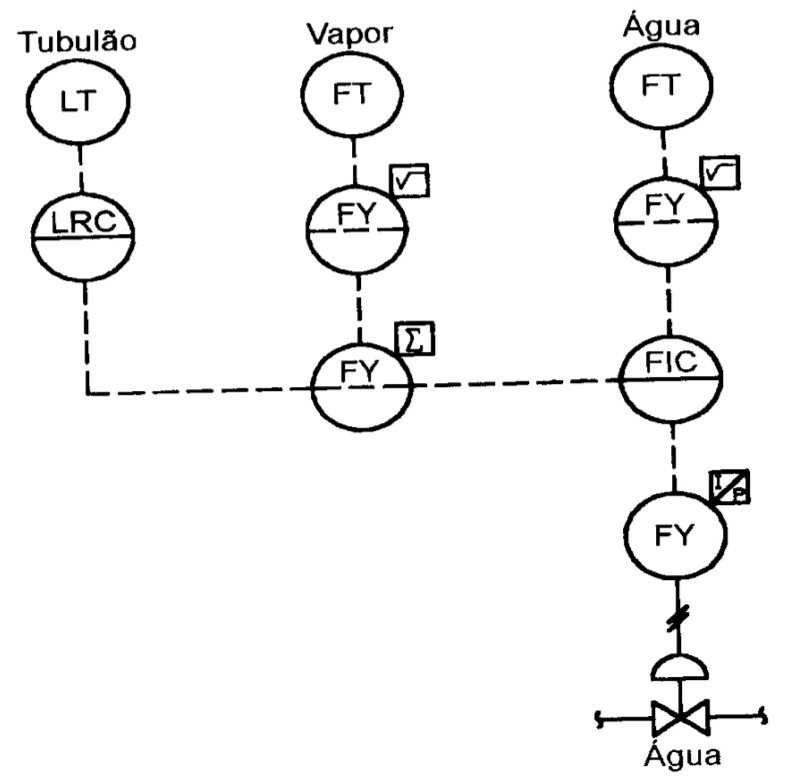
\includegraphics[scale=.35]{img/malha_3_eltos.png}
  \end{center}
  \legend{Fonte: \citeonline{ufrj}}
\end{figure}

As seguintes siglas são utilizadas (legenda retirada de
\citeonline{isa-1984}):

\begin{itemize}
\item \textbf{LT} (transmissor de nível): Captura o nível do tubulão e
  transmite para uma unidade de processamento;
\item \textbf{FT} (transmissor de vazão): Captura a vazão e transmite
  para uma unidade de processamento;
\item \textbf{LRC} (controlador de nível): Recebe o sinal de nível e
  gera um sinal de controle na saída;
\item \textbf{FY} (dispositivo de cálculo): Realiza cálculos baseados
  na entrada e sua função. As seguintes funções foram usadas na
  malha:
  \begin{itemize}
  \item Para o símbolo $\sqrt{\phantom{x}}$, calcula-se $Y=\sqrt{X}$;
  \item Para o símbolo $\Sigma$, calcula-se $Y=\sum_{i} X_i$;
  \item para o símbolo $^I/_P$, o bloco transforma o sinal de corrente
    em um sinal pneumático;
  \end{itemize}
  Onde $X$ é a entrada e $Y$ a saída no bloco;
\item \textbf{FIC} (controlador de vazão): Com base nos sinais de
  entrada, gera um sinal de controle a ser aplicado na válvula de saída
\end{itemize}

No caso, o FIC e o FY com símbolo $^I/_p$ estão contidos no modelo da
válvula de controle de vazão de entrada de água. Teoricamente,
portanto, seriam necessários modelos de válvulas tanto para a entrada
de água quanto para a saída de vapor. Um bom modelo seria capaz de
mostrar as perdas de pressão e o comportamento dinâmico da vazão
durante o acionamento da válvula.

\subsection{Controle de pressão}

Em caldeiras de vapor, normalmente a pressão é mantida em torno de um
valor constante, capaz de suportar a carga máxima para a qual a
caldeira foi projetada \cite{brantly1942steam}. Esse controle da
pressão é feito através da alteração do fluxo de calor entregue à
caldeira: para se aumentar a pressão, basta aumentar o fluxo de calor
entregue. Como demonstrado em \cite{controle-pressao}, um controle
proporcional-integral é suficiente para tal.

\begin{figure}[htb]
  \caption{\label{blocospressao} Diagrama de blocos do controle de
    pressão de uma caldeira}
  \begin{center}
    \begin{tikzpicture}[auto, node distance=2cm,>=latex']
        % We start by placing the blocks
        \node [input, name=input] {};
        \node [sum, right of=input] (sum) {};
        \node [block, right of=sum] (controller) {PI};
        \node [block, right of=controller, node distance=3.2cm] (queimador) {Queimador};
        \node [block, right of=queimador, node distance=3.2cm]
        (caldeira) {Caldeira};
        \node [output, right of=caldeira] (output) {};
        \coordinate [below of=controller] (tmp);
            
        % Once the nodes are placed, connecting them is easy.
        \draw [draw,->] (input) -- node {$p_u$} (sum);
        \draw [->] (sum) -- node {$e$} (controller);
        \draw [->] (controller) -- node {$Q_u$} (queimador);
        \draw [->] (queimador) --node {$Q$} (caldeira);
        \draw [->] (caldeira) --node [name=out] {$p$} (output);
        \draw [->] (out) |- (tmp) -| node[pos=.99] {$-$} (sum);
    \end{tikzpicture}
  \end{center}
\end{figure}


\subsection{Trocas de mensagens entre processos}

Em arquiteturas de software distribuídas, a troca de informações entre
os processos é essencial. Essa troca de informações usa protocolos de
comunicação comuns e é chamada de \textit{comunicação inter-processos}
\cite{wikiipc}. Os processos podem estar na mesma máquina física ou em
localidades separadas, podendo usar vários protocolos diferentes para
a comunicação, desde TCP/IP até pipes de sistemas POSIX.

Tendo a comunicação inter-processo em mente, o sistema de filas de
mensagens (\textit{Message Queueing System}, abreviado por
\textit{MQ}) é usado. Um MQ é um sistema que disponibiliza uma
interface aos processos para que os mesmos possam trocar mensagens
entre si \cite{feldbaum2002method}. Esse sistema é gerenciado por um
processo externo e várias implementações disponibilizam serviços como
balanceamento de carga, ordenação das mensagens (por prioridade ou
FIFO, por exemplo) e mecanismos de segurança para troca de mensagens.

\subsubsection{Padrões de mensagens}
Padrões de mensagens são a forma com que o os nós da comunicação irão
consumir e gerar mensagens, sendo cada padrão adequado a um problema
\cite{zmq}. Para o trabalho proposto, apenas dois dos padrões
disponíveis foram utilizados. Ambos estão explicados nas seções a
seguir.

\subsubsubsection{Padrão request-reply}

O padrão request-reply é o padrão mais simples. Nele, existe um
servidor e um cliente, de tal forma que o segundo envia mensagens de
requisição ao primeiro. Ao receber uma requisição, o servidor responde
com outra mensagem. Um servidor pode receber mensagem de vários
clientes, mas um cliente só envia mensagem para um servidor por vez.

\subsubsubsection{Padrão push-pull}

No padrão push-pull não há entidades cliente-servidor. Ao invés disso,
existe o produtor e o consumidor, onde o produtor envia mensagens ao
consumidor. O consumidor não irá responder, mas pode continuar
enviando o resultado do processamento da mensagem recebida ao próximo
consumidor do fluxo, tornando-se o produtor da nova relação. Pode
existir uma associação de vários produtores enviando mensagens para um
consumidor ou vários consumidores recebendo mensagem de um único
produtor.


\section{Metodologia}
\subsection{Propriedades termodinâmicas da água}
Todas as aproximações foram obtidas em \citeonline{garland} e apesar
de serem restritas a uma faixa de pressão, outros valores próximos aos
limites dessa faixa podem ser extrapolados através de métodos
númericos. As derivadas dessas variáveis em relação à pressão foram
calculadas analiticamente, dentro de cada faixa contínua.

As funções implementadas foram testadas usando tabelas de vapor
saturado obtidas de \citeonline{ufrj}, conforme mostrado na figura
\ref{plots_steam_tables}.

\begin{figure}[H]
\caption{\label{plots_steam_tables} Comparação de aproximações das
  propriedades termodinâmicas da água}
\begin{center}
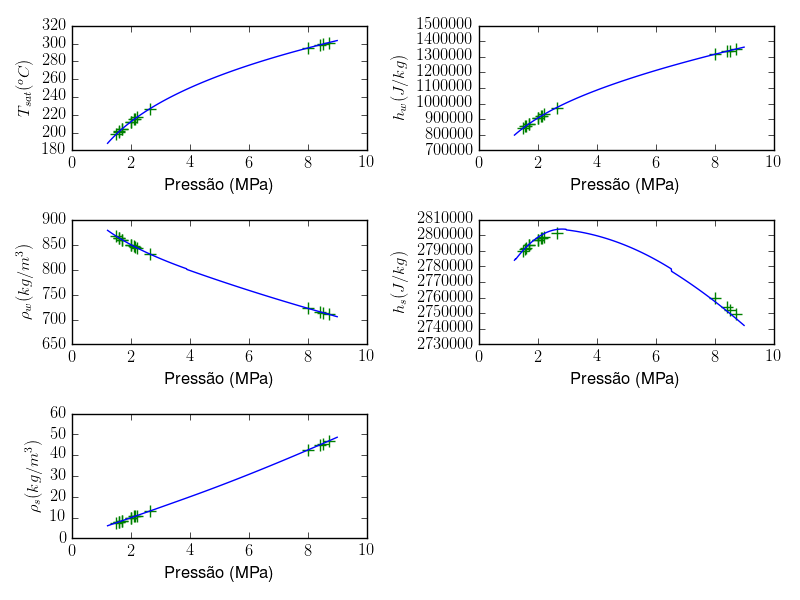
\includegraphics[scale=0.7]{img/steam_table_plots.png}
\end{center}
\legend{As linhas são valores aproximados, enquanto as cruzes
  representam os valores encontrados nas tabelas de vapor saturado}
\end{figure}

O maior erro relativo encontrado foi de cerca de $2,6\%$, mas as
simulações mostraram que esse erro é irrelevante para o comportamento
dinâmico do mesmo.


\subsection{Parâmetros de simulação}

Para a configuração do simulador em relação a uma determinada
caldeira, parâmetros devem ser estimados. Dentre eles, pode-se citar
aspectos geométricos da caldeira e dados da caldeira em seu ponto de
operação ideal. Os tópicos a seguir apresentam uma forma de calcular
tais parâmetros quando em posse de uma caldeira em funcionamento. O
fluxo de cálculo das estimativas foi definido levando em consideração
a dificuldade de se mensurar valores complexos relacionados à
termodinâmica e à geometria da caldeira.

Recomenda-se que os cáculos sejam feitos na ordem em que estão
apresentados, uma vez que as variáveis possuem dependências entre si.

\subsubsection{Gravidade ($g$)}

Esse parâmetro pode ser escolhido arbitrariamente, em torno da
gravidade usual. Os gráficos a seguir mostram as respostas do
simulador a um degrau de $10kg/s$ em $q_s$ para a gravidade entre
$80\%$ e $110\%$ da estimativa original.

\begin{figure}[H]
  \caption{\label{level_resp_g} Respostas do nível a degrau de $10kg/s$
    em $q_s$ para gravidade em variações diferentes}
  \centering
  \subbottom[\label{level_resp_g:80}$80\%$]{
    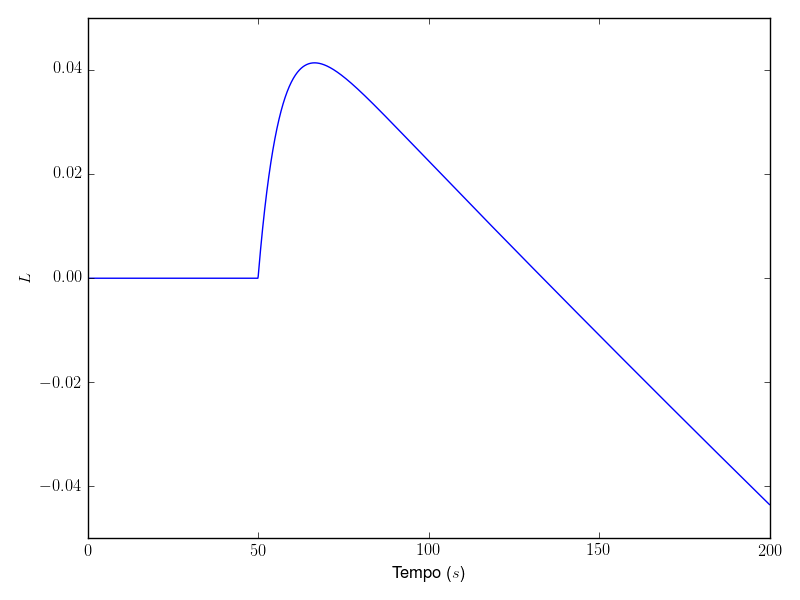
\includegraphics[scale=.25]{img/level_response_test_g_80.png} }
  \subbottom[\label{level_resp_g:90}$90\%$]{
    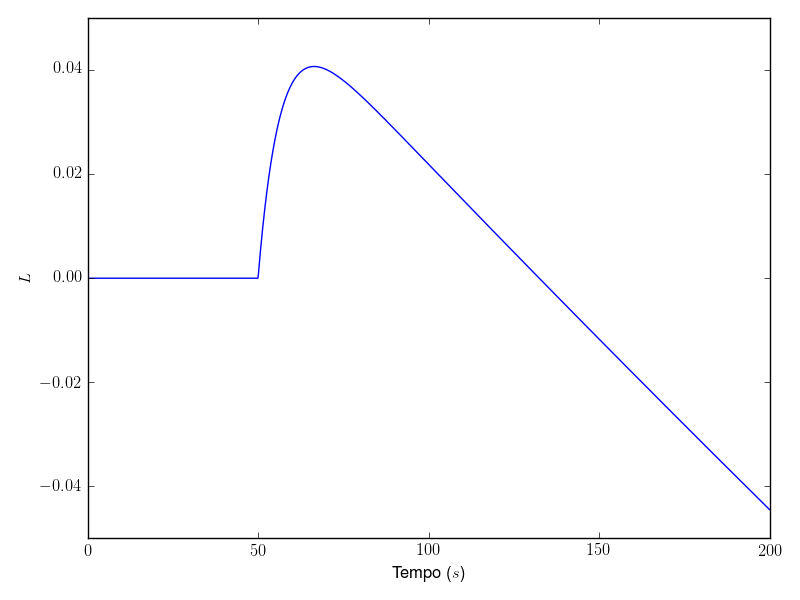
\includegraphics[scale=.25]{img/level_response_test_g_90.png} }
  \subbottom[\label{level_resp_g:110}$110\%$]{
    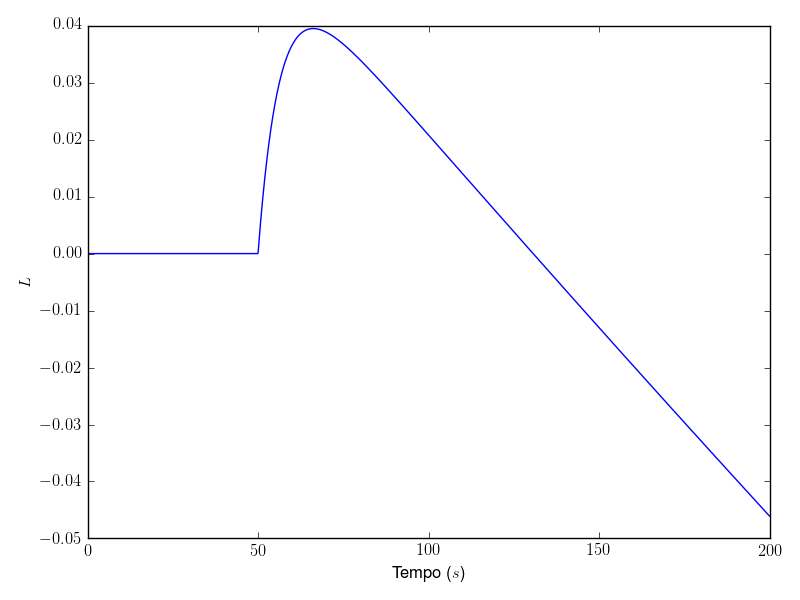
\includegraphics[scale=.25]{img/level_response_test_g_110.png} }
  \subbottom[\label{level_resp_g:120}$120\%$]{
    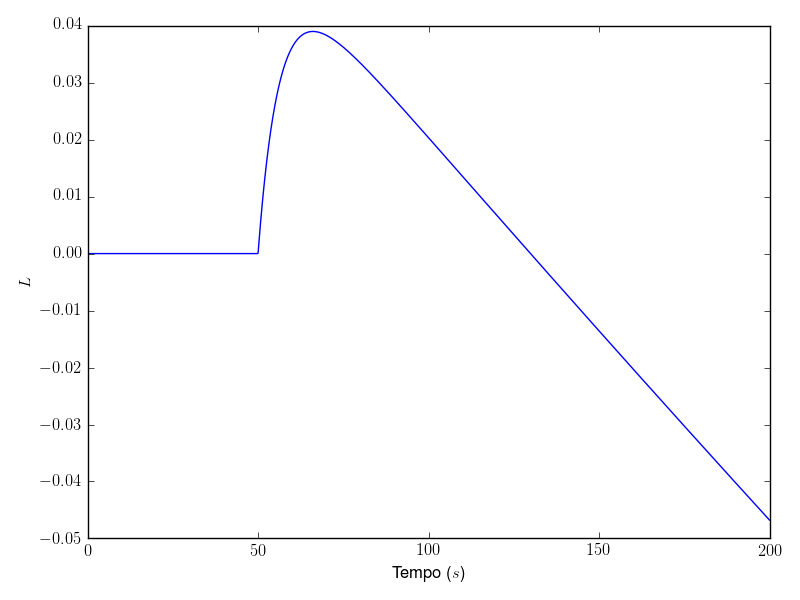
\includegraphics[scale=.25]{img/level_response_test_g_120.png} }
\end{figure}

A seguir, as figuras mostram a resposta de outras variáveis da
caldeira ao mesmo degrau de $10kg/s$ em $q_s$.

\begin{figure}[H]
  \caption{\label{resp_g} Respostas de variáveis de estado a degrau de
    $10kg/s$ em $q_s$ para gravidade em variações diferentes}
  \centering \subbottom[\label{resp_g:80}$80\%$]{
    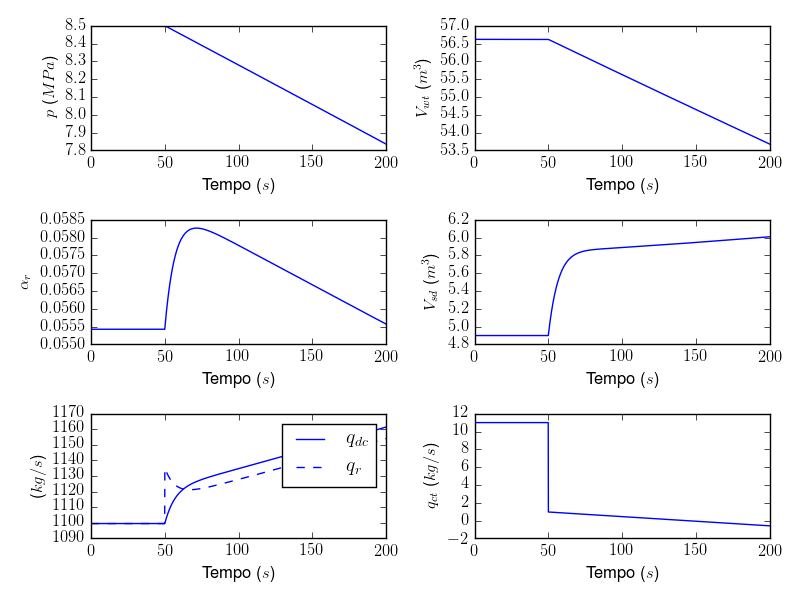
\includegraphics[scale=.25]{img/response_test_g_80.png} }
  \subbottom[\label{resp_g:90}$90\%$]{
    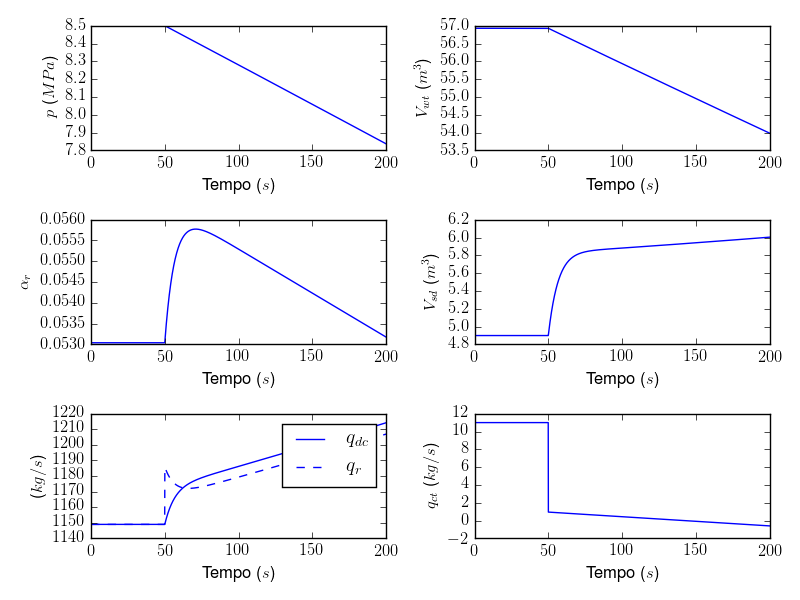
\includegraphics[scale=.25]{img/response_test_g_90.png} }
  \subbottom[\label{resp_g:110}$110\%$]{
    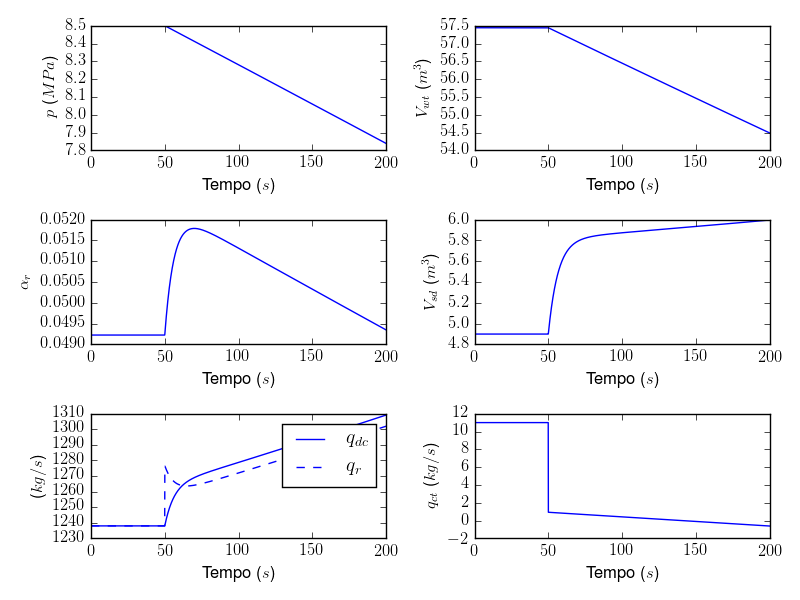
\includegraphics[scale=.25]{img/response_test_g_110.png} }
  \subbottom[\label{resp_g:120}$120\%$]{
    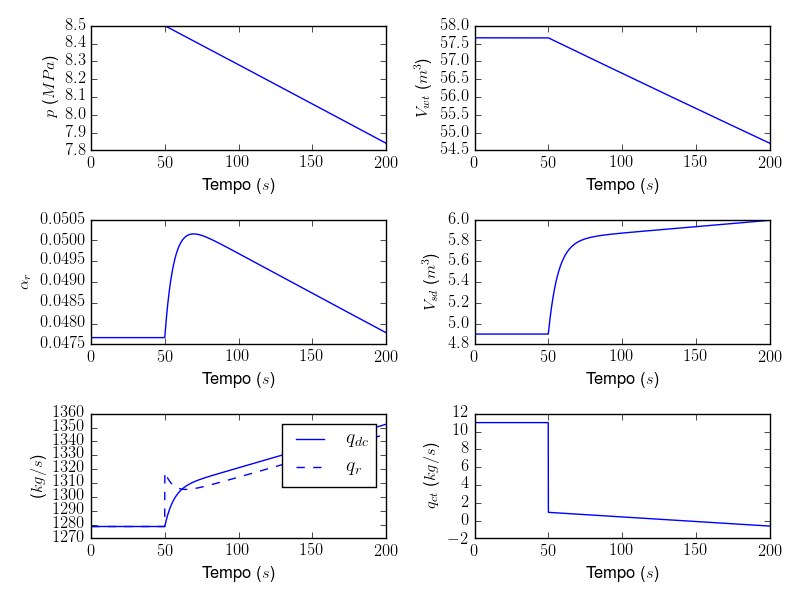
\includegraphics[scale=.25]{img/response_test_g_120.png} }
\end{figure}

Como pode ser visto, a variação do valor da gravidade não afeta em
nada o comportamento dinâmico do sistema. Os valores iniciais são
afetados pois foram estimados inicialmente usando um valor fixo para a
gravidade, porém se os valores iniciais fossem reestimados com a
variação da gravidade, seriam coincidentes com os valores encontrados
em \citeonline{astrom}.

\subsubsection{Entalpia da água de entrada ($h_f$)}

Para baixas temperaturas e altas pressões, as propriedades
termodinâmicas da água são governadas por sua temperatura
\cite{garland2}. No caso das propriedades da água de entrada, pode-se
usar sua temperatura para descobrir a pressão de saturação, através
das aproximações em \citeonline{garland2}. Pode-se então usar essa
pressão de saturação nas aproximações para a água superaquecida,
explicadas em \citeonline{garland}.

\subsubsection{Volume total de água na caldeira ($V_{wt}$)}

Com o valor de $l_o$ obtido da caldeira e o valor inicial de $V_{sd}$
calculado com a equação de $V_{sd}$ no sistema \ref{sistema_geral_rp},
pode-se calcular $V_{wd}$ através da equação \ref{nivel_agua}.

\begin{center}
  $l_o = \dfrac{V_{wd} + V_{sd}}{A_d} \Rightarrow V_{wd} = l_o  A_d -
  V_{sd}$
\end{center}

Com o valor de $V_{wd}$, basta usar a equação \ref{V_wd} para
encontrar $V_{wt}$.



\subsection{Estimativas da caldeira de \citeonline{astrom}}

Além dos parâmetros citados em \citeonline{astrom}, outros são
necessários e foram omitidos em seu trabalho. Tais parâmetros foram
estimados a partir da figura \ref{plots_astrom_step_10kg_qs}.

\begin{figure}[H]
  \caption{\label{plots_astrom_step_10kg_qs} Respostas a incremento de
  $10 kg/s$ na vazão mássica de vapor, a partir de carga média}
  \begin{center}
    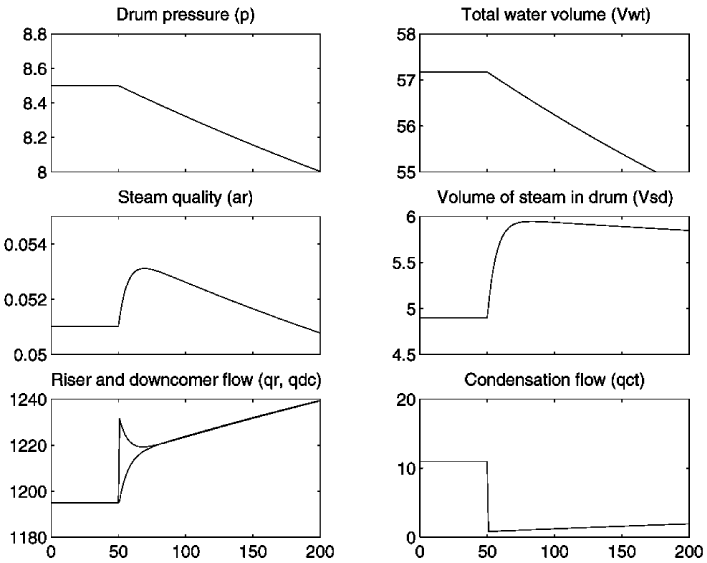
\includegraphics[scale=0.45]{img/plots_astrom_step_q_s_10kg.png}
  \end{center}
  \legend{Fonte: \cite{astrom}. }
\end{figure}

Pode-se retirar da figura os seguintes valores iniciais:
\begin{itemize}
\item $ p = 8,5 MPa $
\item $ V_{wt} = 57,2 m^3 $
\item $ \alpha_r = 0,051 $
\item $ V_{sd} = 4,9 m^3 $
\item $ q_r = q_{dc} = 1190 kg/s $
\item $ q_{ct} = 11 kg/s $
\end{itemize}

Através da pressão inicial e das aproximações das tabelas de vapor
saturado, pode-se calcular o valor das propriedades térmicas da água.

\begin{itemize}
\item $h_s = 2.749.993,696 J/kg$
\item $h_w = 1.340.249,233 J/kg $
\item $h_c = 1.409.744,462 J/kg$
\item $\rho_s = 45,627 kg/m^3$
\item $\rho_w = 713,847 kg/m^3$
\end{itemize}

\subsubsection{Vazão de entrada ($ q_f $)}

Através do sistema de equações \ref{sistema_geral_rp}, pode-se
encontrar o valor de $Q$ inicial, ao utilizar o valor de $h_c$ obtido
das aproximações das tabelas de vapor saturado, juntamente com os
valores de $q_{dc}$ e $\alpha_r$ iniciais observados no gráfico de
\citeonline{astrom}:

$Q = 1195 \times 0,051 \times 1.409.744,4622785489 = 85.916.876,2536
W$

Através do sistema de equações \ref{sistema_geral_rp}, da equação em
regime permanente de $q_{ct}$ e dos valores iniciais obtidos dos
gráficos, pode-se estimar a vazão mássica inicial usada:


\begin{center}
  $Q = q_s h_s - q_f h_f \Rightarrow Q = q_f h_s - q_f h_f$
\end{center}

\begin{equation}  
  q_f h_f = q_f h_s - Q
  \label{qfhf1}
\end{equation}

A partir da equação de $q_{ct}$, tem-se:

\begin{center}
  $q_{ct} = \dfrac{h_w - h_f}{h_c} q_f$

  $q_{ct} h_c = q_f h_w - q_f h_f$
\end{center}

\begin{equation}
  q_f h_f = q_w h_w - q_{ct} h_c
  \label{qfhf2}
\end{equation}

Igualando \ref{qfhf1} e \ref{qfhf2}, obtém-se o valor de $q_f$:

\begin{equation}
  q_f=\dfrac{q_{ct} h_c - Q}{h_w - h_s}
  \label{q_f_init}
\end{equation}

No caso do simulador em questão, esse valor é igual a $q_f = 49,945
kg/s$.

\subsubsection{Entalpia da água de entrada ($h_f$)}

Por não ser mencionada a temperatura da água de entrada em
\citeonline{astrom}, a mesma foi estimada a partir do $Q$ inicial,
substituindo-o na segunda equação do sistema \ref{sistema_geral_rp}.

\begin{center}
  $Q = q_s h_s - q_f h_f \Rightarrow h_f = \dfrac{q_s h_s - Q}{q_f} =
  \dfrac{49.945 \times 2749993,6956 - 85.916.876,2536}{49.945}$
  
  $\therefore h_f = 1.029.763,918 J/kg$
\end{center}

\subsubsection{Área dos tubos descendentes ($A_{dc}$)}

A partir do valor inicial de $\alpha_r$, obtém-se o valor de
$\bar{\alpha}_v$:

\begin{center}
  $\bar{\alpha}_v = 0,2704784 $
\end{center}

Inserindo os valores na equação \ref{Q_lin_sys}, obtém-se o seguinte
valor:

\begin{center}
  $A_{dc} = \dfrac{ k Q^2 }{ 2 \alpha_r^2 h_c^2 \rho_w (\rho_w - \rho_s)
    g \bar{\alpha}_v V_r}  = 0,381657338 m^2$
\end{center}

Os valores iniciais para o restante das variáveis haviam sido
calculados conforme explicado anteriormente, usando as equações de
\ref{sistema_geral_rp} e \ref{Q_lin_sys}.

\subsubsection{Volume de vapor no tubulão para situação hipotética sem
  condensação ($V_{sd}^0)$}

A partir do valor inicial de $V_{sd}$ no gráfico, pode-se estimar o
valor de $V_{sd}^0$ da caldeira ao substituir o valor na equação de
$V_{sd}$ no sistema de equações \ref{sistema_geral_rp}:

\begin{center}
  $V_{sd} = V_{sd}^0 - \dfrac{T_d ( h_w - h_f )} {\rho_s h_c} q_f
  \Rightarrow V_{sd}^0 = V_{sd} + \dfrac{T_d ( h_w - h_f )} {\rho_s
    h_c} q_f$

  $ \therefore V_{sd}^0 = 7,7930138 m^3 $  
\end{center}

\subsubsection{Volume total da caldeira ($V_t$)}

Embora não especificado em \citeonline{astrom}, estima-se que o volume
total da caldeira pode ser representado através dos parâmetros de
entrada do sistema:

\begin{equation}
  V_t = V_d + V_{dc} + V_r = 89 m^3
  \label{V_t_params}
\end{equation}

\subsubsection{Nível da água no ponto de operação ($l_o$)}

Usando o valor inicial de $V_{wt}$, pode-se calcular $V_{wd}$ através
da equação \ref{V_wd}, obtendo um valor de $19,205 m^3$. Sabe-se que,
no ponto de operação, $l=l_w=l_s=0$, então basta usar as equações
\ref{nivel_agua}, \ref{contrib_s_nivel} e \ref{contrib_w_nivel}:

\begin{center}
  $l_{wo} = \dfrac{V_{wd}}{A_d} = 0,9603 m$
  
  $l_{so} = \dfrac{V_{sd}}{A_d} = 0,2450 m$
  
  $l_o = l_{wo} + l_{so} = 1,2053 m$
\end{center}

Para a utilização prática do simulador, esse valor deve ser obtido
através da medição da caldeira original, uma vez que $V_{wd}$ é obtido
através do valor de $l_o$. Esse fluxo de cálculos foi escolhido pois
caldeiras podem ter geometrias complicadas, o que dificulta o cálculo
preciso de volumes \cite{astrom}.

\subsection{Válvula de vazão de água}

Um modelo simples com controle proporcional foi adotado para as
válvulas, eliminando o comportamento instantâneo na mudança de vazão
de vapor e água de alimentação. Também foi adotado um gerador de
distúrbios de acordo com uma distribuição normal. Na figura
\ref{valvulas_step} pode-se ver a resposta do modelo com e sem distúrbio.

\begin{figure}[H]
  \caption{\label{valvulas_step} Resposta do modelo da válvula a um
    degrau de $10kg/s$}
  \centering
  \subbottom[\label{valvulas_step:sem_d} Sem distúrbio]{
    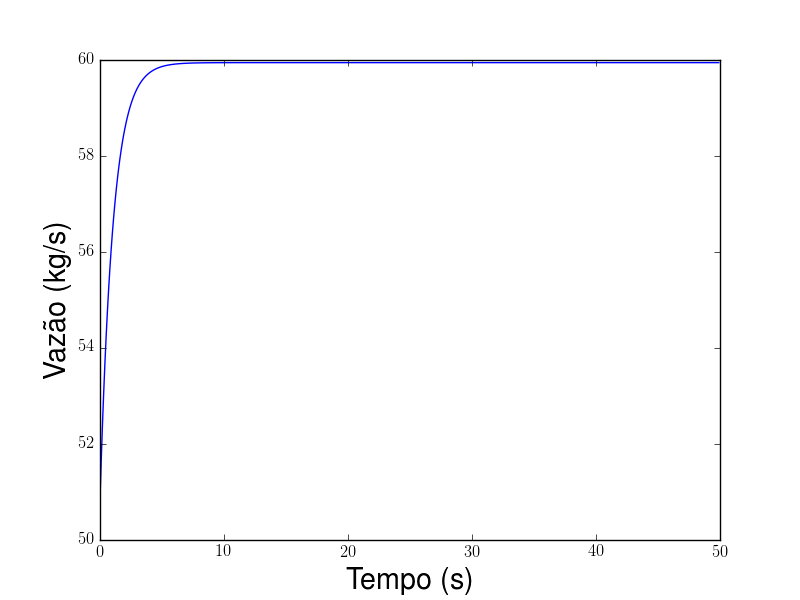
\includegraphics[scale=.25]{img/valve_step_response.png}}
  \subbottom[\label{valvulas_step:com_d} Distúrbio de $\pm 0,3 kg/s$]{
    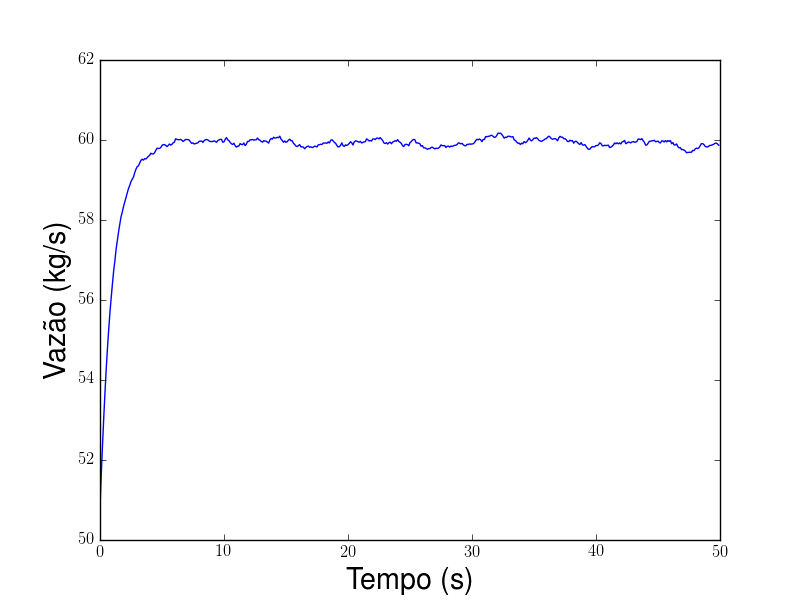
\includegraphics[scale=.25]{img/valve_step_response_biased.png}}
\end{figure}

Claramente uma válvula tem um limite de vazão possível. Para esse
trabalho a vazão máxima escolhida foi de $130,00 kg/s$, levando em
conta os gráficos para a caldeira em operação com carga alta, expostos
em \citeonline{astrom}.

\subsection{Dinâmica da geração de calor}

Para um simulador condizente com a realidade, é necessário simular o
comportamento do sistema para estímulos no fluxo de calor fornecido
para a planta ($Q$). Por se tratar de um comportamento dependente do
modelo dos queimadores da caldeira, o modelo do queimador deve ser
usado, com um sistema de controle próprio. Como a implementação de tal
modelo foge ao escopo do projeto, um simples modelo linear para o
fluxo de calor foi adotado, considerando uma relação linear entre o
fluxo mássico de combustível e o fluxo de calor entregue à caldeira,
apresentado na equação \ref{modelo-calor}. Na fórmula, $k$ foi
escolhido empiricamente, de forma a aproximar-se da constante de tempo
vista nos dados originais obtidos em \citeonline{astrom}. Um valor de
$k = 0,1$ se mostrou satisfatório.

\begin{equation}
  \dot{Q}(t) = Q(t) + k(u - Q(t))
  \label{modelo-calor}
\end{equation}

No caso, $u$ é o ponto de referência para $Q$. Tal modelo causa um
atraso na resposta da $Q$, aproximando-se a modelos de queimadores
reais.

\subsection{Sistemas de controle}

Os dois sistemas de controle principais da caldeira são o controle de
nível e controle de pressão. Como dito em \citeonline{ufrj}, muitas
vezes os dois controles são analisados separadamente, realizando o
ajuste do controle de pressão e depois o ajuste do controle de nível.

\subsubsection{Controle de pressão}

Empiricamente, as seguintes constantes foram adotadas no controlador
PI da pressão:

\begin{equation}
  \begin{cases}
    k_p = 5\times10^6\\
    k_i = 10^7\\
  \end{cases}
  \label{ks_pi_pressao}
\end{equation}

A pressão adotada foi a inicial encontrada nos gráficos em
\citeonline{astrom}, para a caldeira trabalhando com carga média:
$8,5 MPa$.

\subsubsection{Controle de nível}

De acordo com \citeonline{adam1999} e \citeonline{ufrj}, um
controlador PI é suficiente para controlar o nível de água no tubulão,
porém mostra-se complicado o ajuste de tais parâmetros de forma
ótima. Aqui, portanto, usou-se o método prático estabelecido por
\citeonline{ufrj}, que consiste na estimativa empírica dos parâmetros
do controlador após o ajuste do controlador de pressão. Os resultados
do ajuste prático encontram-se a seguir.

\begin{equation}
  \begin{cases}
    k_p=60\\
    k_i=1,2
  \end{cases}
  \label{ks_pid_agua}
\end{equation}

\subsection{Arquitetura de software}

Para se aproximar ao máximo da arquitetura lógica de uma caldeira
real, optou-se por desenvolver um sistema distribuido, em que cada uma
das partes seja facilmente removida. Isso também permite que cada
aplicação seja independente, podendo ser desenvolvida em uma linguagem
diferente da linguagem usada por outras aplicações.

No centro dessa arquitetura, há o simulador do sistema, onde se tem
implementado o modelo da caldeira, assim como os modelos da válvula de
entrada de água e dos queimadores. A implementação desses modelos
podem ser vistos nos anexos \ref{sim_caldeira}, \ref{sim_valvula} e
\ref{sim_queimador}, respectivamente.

O simulador apresenta serviços acessíveis através de sua interface,
onde se pode requisitar os valores de cada variável da caldeira, bem
como alterar valores das mesmas. As variáveis controladas diretamante
através dessa interface são $q_s$, $q_f$ (que na verdade é passada
para o controlador da válvula), e $Q$ (passado para o controlador dos
queimadores), enquanto as variáveis que podem ser lidas são $q_f$,
$q_s$, $Q$, $L$, $P$ e $\alpha_r$. Os anexos \ref{sim_main} e
\ref{sim_thread} mostram o módulo de entrada do simulador e a thread
de controle da simulação.
% TODO: Adicionar apendices

Para fins de testes do simulador, as seguintes aplicações foram
desenvolvidos:
\begin{itemize}
  \item \textbf{Ferramenta de visualização}: Interface gráfica onde
    pode-se ver um gráfico de todas as variáveis disponíveis através
    da interface. A implementação resume-se em um único módulo, que
    pode ser visto no anexo \ref{viewer_main}.
  \item \textbf{Controladores}: Aplicação que implementa os controladores
    de pressão e nível.
\end{itemize}

A aplicação de controladores é constituída do ponto de entrada (módulo
\textit{main}, disponível no anexo \ref{controllers_main}, uma classe
para controle de nível e outra para controle de pressão. Os
controladores usados fazem parte de um módulo de classes de
controladores base, como podem ser vistos em
\ref{controllers_generic}. As classes de controle de nível e controle
de pressão são instanciadas em \textit{main} e realizam o controle
periodicamente, através do método \textit{step}. A implementação de
ambas as classes está disponível nos anexos \ref{controllers_level} e
\ref{controllers_pressure}.


Outro fator de extrema importância em sistemas distribuidos é a
comunicação entre os processos. Para isso, foi usado o
\textit{ZeroMQ}, um MQ que disponibiliza sockets que carregam
mensagens entre processos usando protocolos como TCP/IP, multicast,
entre outros \cite{zmq}. O ZeroMQ possui bibliotecas para várias
linguagens, como C++, Python e Matlab.

Para a aplicação, o protocolo escolhido foi TCP/IP, permitindo a
comunicação entre os módulos do sistema mesmo que não estejam no mesmo
computador. A classe usada para comunicação com o servidor está
disponível no anexo \ref{interface_cliente}, enquanto a classe
de interface usada pelo servidor está disponível no anexo
\ref{interface_servidor}.

A interface do servidor conta com dois canais para troca de mensagens,
um funciona como request-reply e o outro como push-pull.

Através do canal request-reply, clientes solicitam os valores das
variáveis. Uma mensagem de requisição deve conter somente o nome da
variável solicitada.

O canal push-pull recebe comandos de alteração das variáveis, seguindo
o formato ``variável operação valor''. A operação pode ser de adição,
subtração, multiplicação ou divisão, representadas pelos símbolos $+$,
$-$, $*$ e $/$. É importante manter o espaço entre cada parte da
mensagem, ou a mesma é considerada inválida e descartada.

Por precisarem de ferramentas numéricas e de plotagem de gráfico, a
linguagem de programação escolhida foi Python, uma linguagem orientada
a objetos de simples utilização e grande suporte da comunidade. As
ferramentas de plotagem (Matplotlib) e bibliotecas numéricas
(SciPy/NumPy) já são maduras e possuem grande aceitação da comunidade
acadêmica.


\section{Resultados}


Todas as aplicações desenvolvidas são inicializadas da mesma forma:
basta executar o módulo ``main'' de cada pacote. Para funcionar, a
aplicação da simulação deve ser chamada primeiro. As telas da
aplicação de visualização e das mensagens do simulador podem ser
vistas nas figuras \ref{pic_viewer} e \ref{pic_sim}, respectivamente.

\begin{figure}[H]
  \caption{\label{pic_viewer} Tela da interface de visualização, após
    aumento de $30\%$ na vazão de vapor}
  \centering
  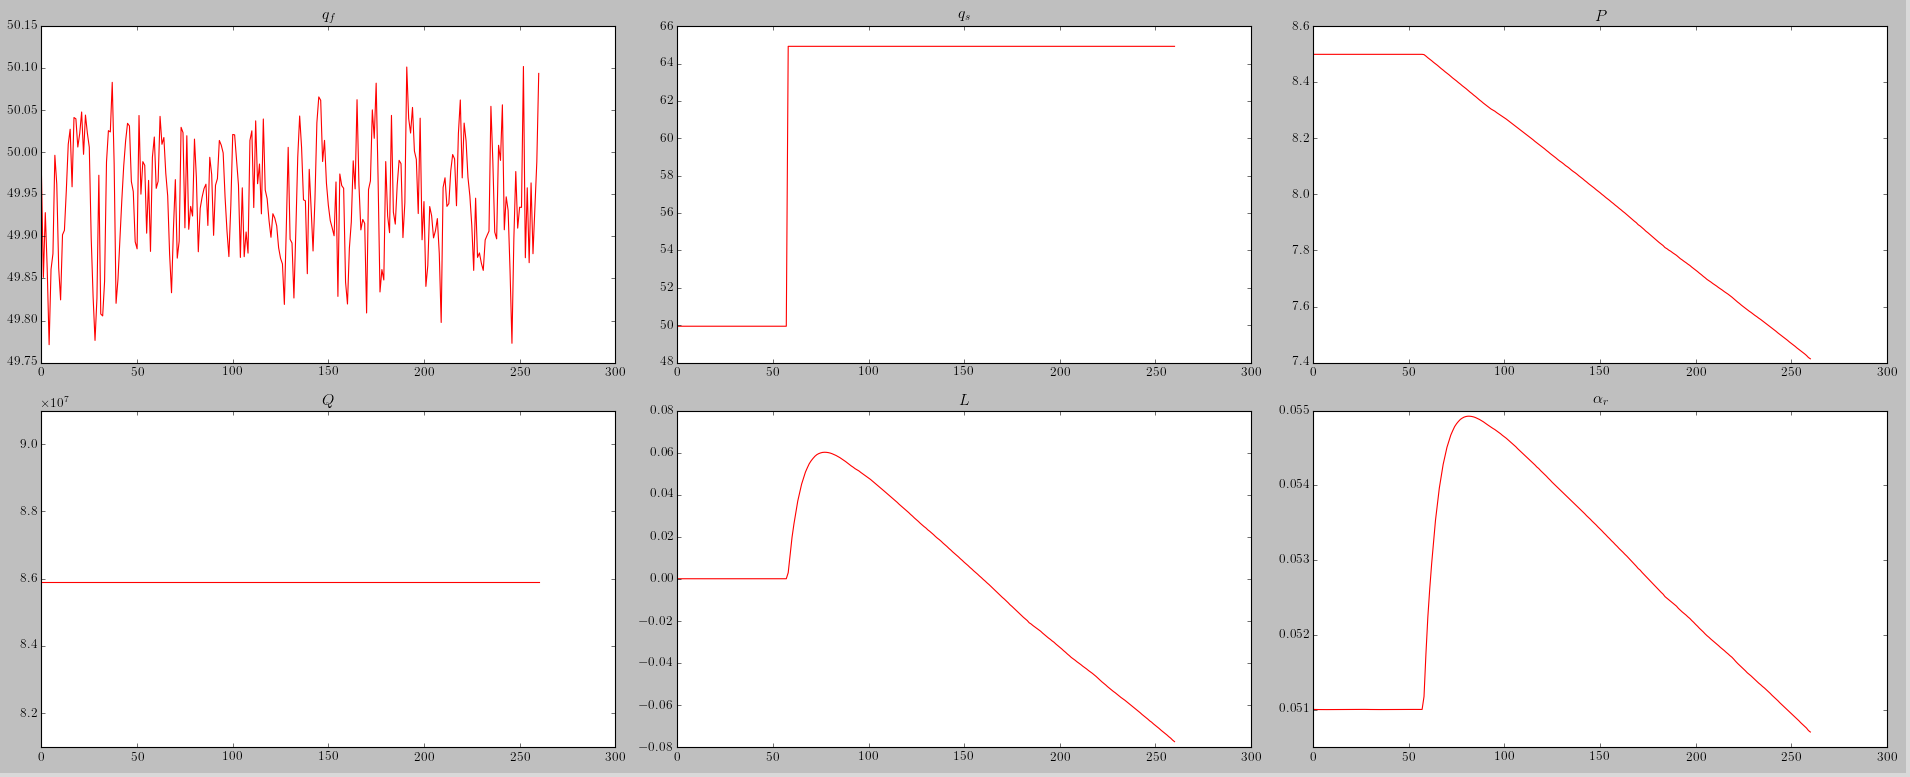
\includegraphics[scale=0.25]{img/pic_viewer.png}
\end{figure}

\begin{figure}[H]
  \caption{\label{pic_sim} Tela do simulador enviando e recebendo
    mensagens}
  \begin{center}
    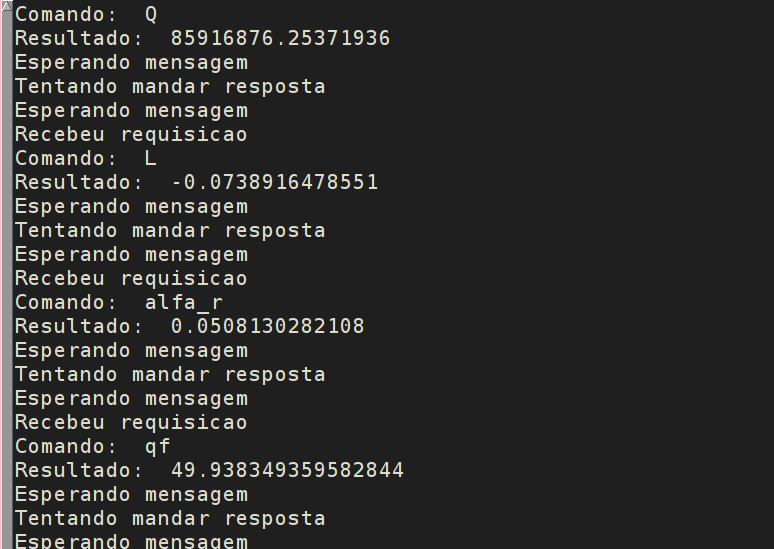
\includegraphics[scale=0.3]{img/pic_sim.png}
  \end{center}
\end{figure}

Na figura \ref{pic_viewer_controllers}, pode-se ver a tela da
interface quando o sistema responde a um aumento de $30\%$ na vazão de
vapor com os controladores ligados. Isso mostra a independência das
aplicações, podendo ativar ou desativar cada uma separadamente, mesmo
com o sistema funcionando.

\begin{figure}[H]
  \caption{\label{pic_viewer_controllers} Tela da interface de
    visualização após aumento de $30\%$ na vazão de vapor, com
    controladores em funcionamento}
  \centering
  \subbottom[\label{pic_viewer_controllers:pressao}Somente controle da
    pressão]{
    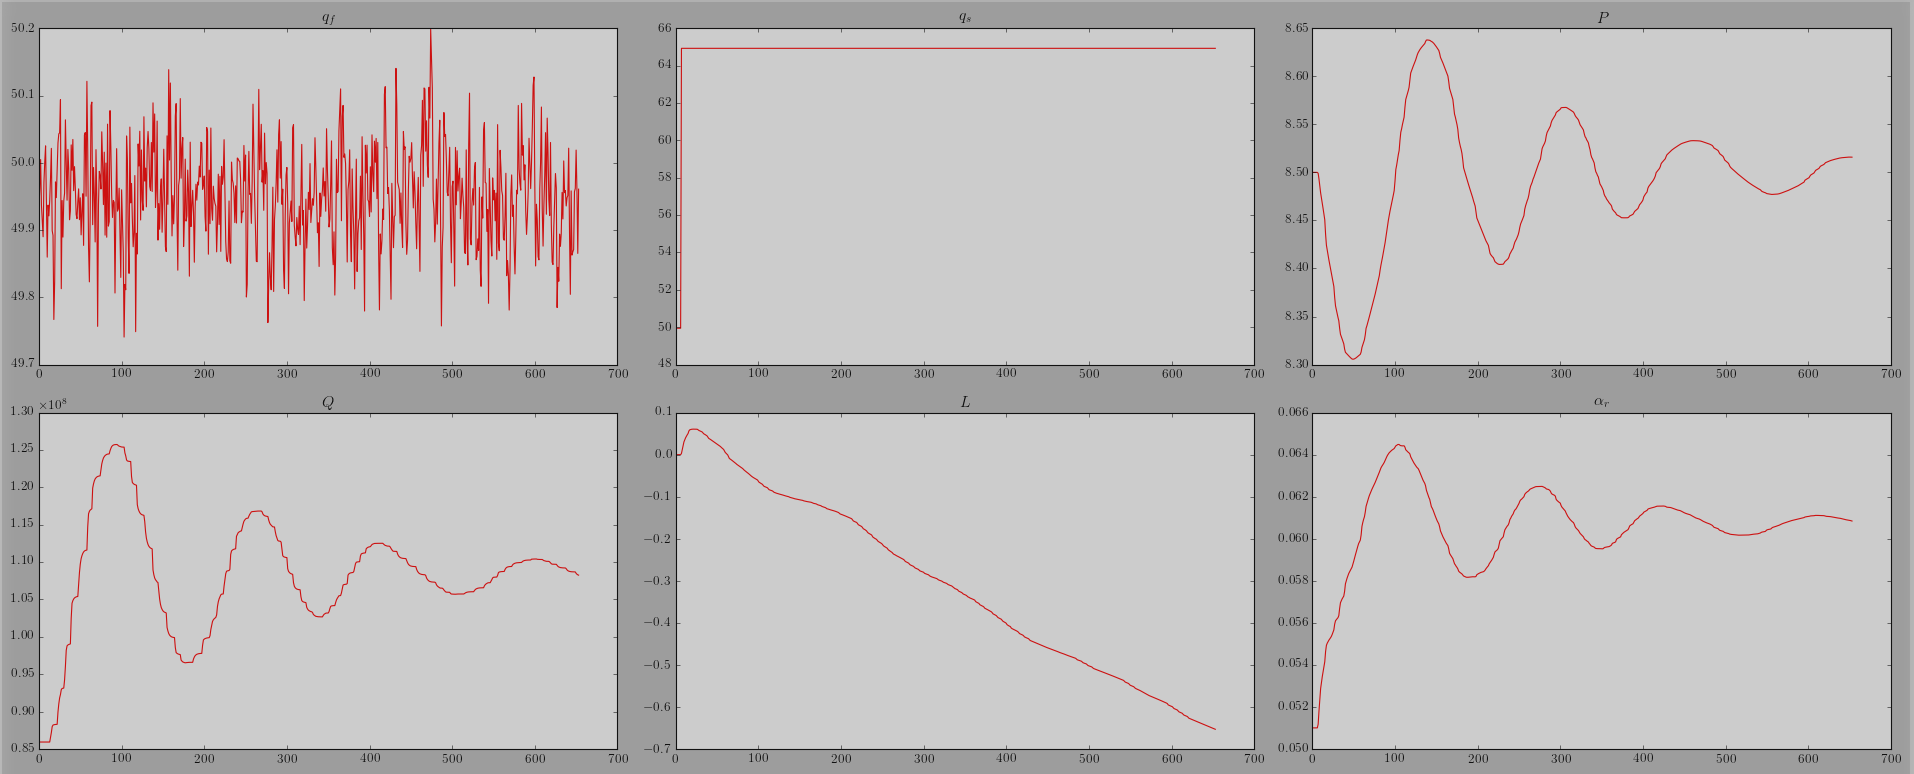
\includegraphics[scale=.25]{img/viewer_contr_pressao.png}}
  \subbottom[\label{pic_viewer_controllers:completo}Controle de
    pressão e nível]{
    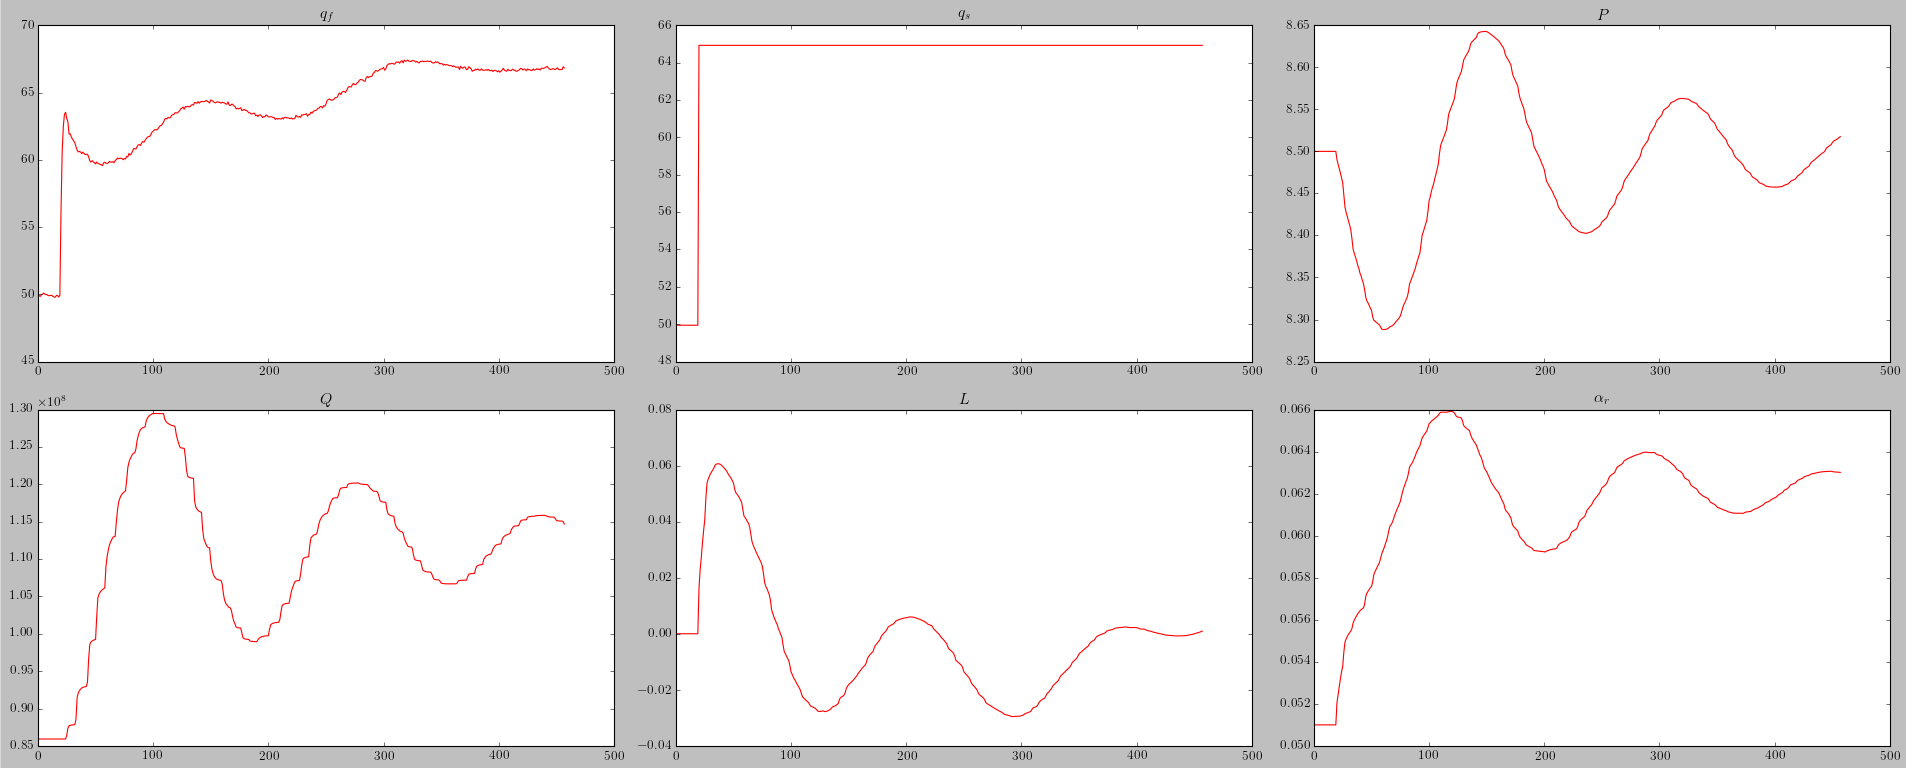
\includegraphics[scale=.25]{img/viewer_controlado.png}}

\end{figure}

Pode-se ver que, apesar de não serem ideais, os controladores são
estáveis, conseguindo ajustar os parâmetros da caldeira corretamente.

Pode-se também usar o console do Python para enviar mensagens usando a
classe de interface cliente, controlando manualmente a planta. A
figura \ref{pic_viewer_zoeira} mostra a reação da planta a vários
estímulos manuais, assim como a tela do console.

\begin{figure}[H]
  \caption{\label{pic_viewer_zoeira} Comportamento da planta ao
    controle manual de parâmetros, com controladores desligados}
  \centering
  \subbottom[\label{pic_viewer_zoeira:console}Console]{
    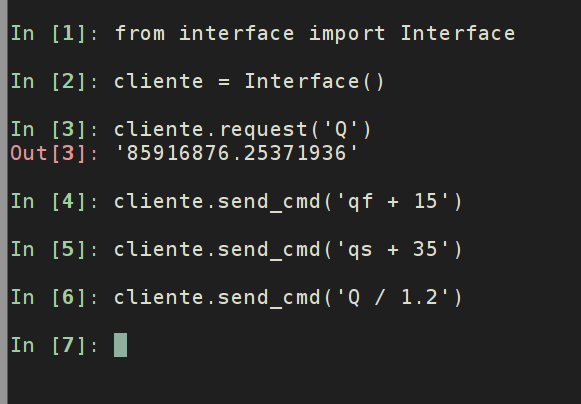
\includegraphics[scale=.25]{img/viewer_zoeira_console.png}}
  \subbottom[\label{pic_viewer_zoeira:viewer}Interface gráfica]{
    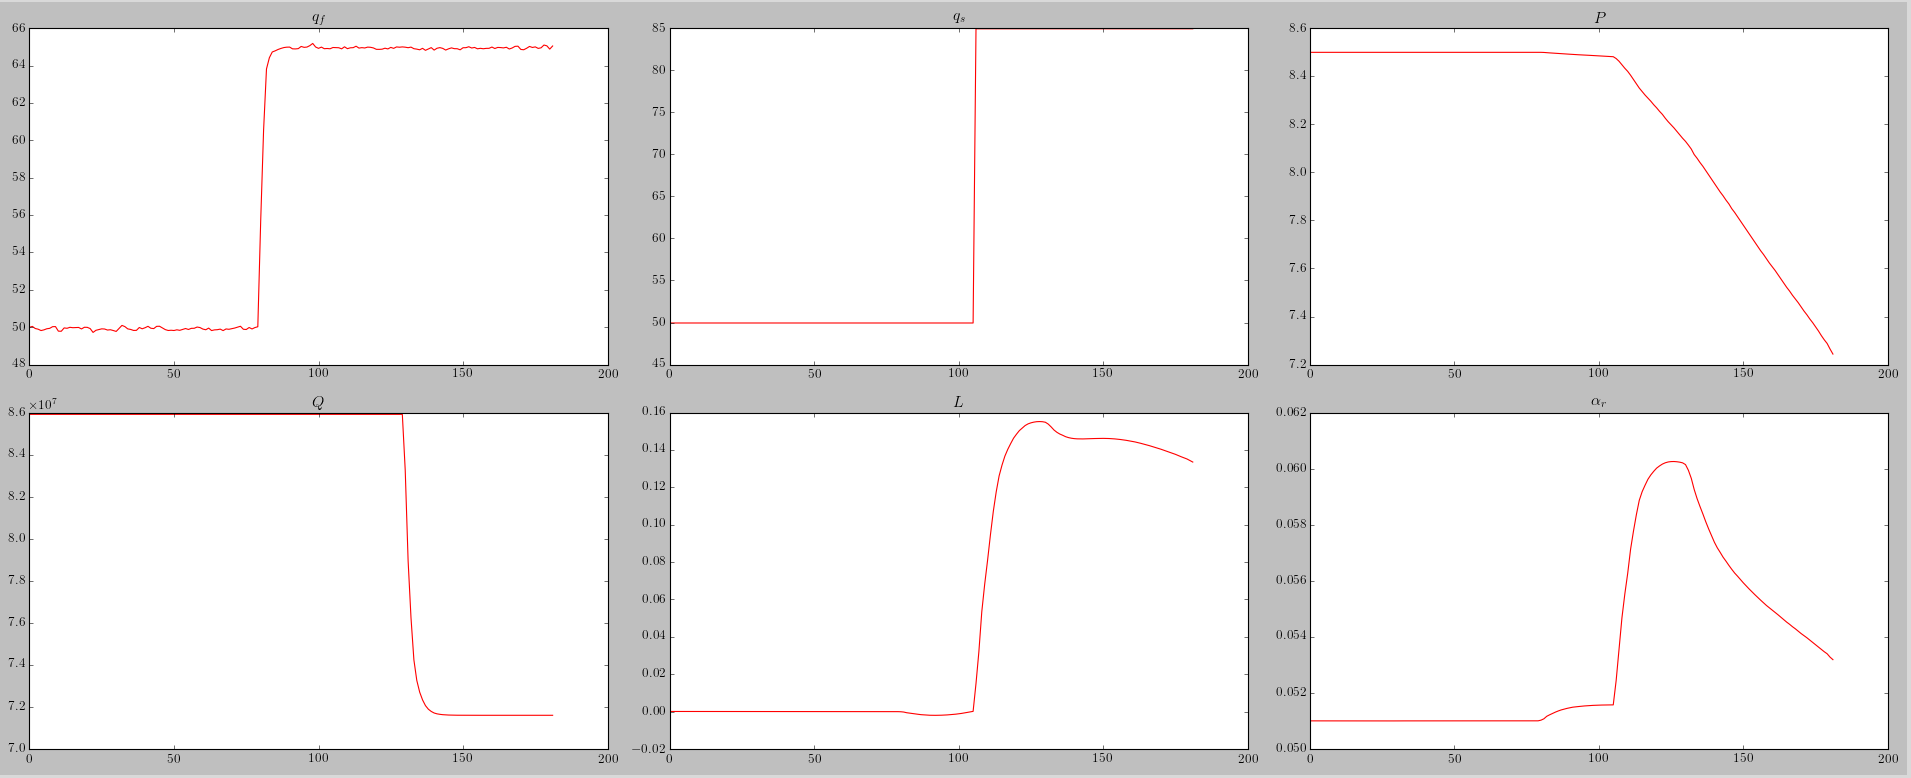
\includegraphics[scale=.25]{img/viewer_zoeira.png}}

\end{figure}



\section{Discussão}
Com a interface funcionando através de um MQ, foi possível simplificar
o desenvolvimento de novos aplicativos que interagem com o
simulador. Isso se mostrou verdadeiro ao se desenvolver tanto os
controladores quanto a interface gráfica. Dessa forma, é possível
agora desenvolver vários outros sistemas baseados no simulador, como
interfaces gráficas para fins educacionais, drivers para comunicação
com CLPs reais, simuladores distribuidos e plataformas colaborativas.

Outras formas de se aumentar a confiabilidade do simulador produzido
seria a implementação de modelos reais para todas as válvulas e para
os queimadores, assim como a adição de parâmetros que aparecem em
sistemas reais, como propensão a erros de medição dos transmissores,
grau de interferência externa, dentre outros. Falta ainda a validação
do simulador com dados de caldeiras de maior potência, onde se usa a
circulação forçada.

Outra forma de se extender o trabalho aqui realizado é desenvolvendo
modelos de plantas que consomem o vapor produzido pela caldeira,
podendo então observar o comportamento do simulador em um ambiente
mais próximo da realidade.



\chapter[Conclusões]{Conclusões}

O objetivo do trabalho foi construir um ambiente de simulação que
possa ser usado no ambiente acadêmico e industrial, possibilitando o
maior entendimento de sistemas de caldeiras aquatubulares e o
comportamento da mesma quando em interação com outros equipamentos. O
simulador provou ser de fácil manuseio, além de apresentar uma
facilidade para se desenvolver aplicações que se comunicam com o
mesmo. Portanto, mostrou-se que o simulador é capaz de cumprir seu
propósito.

Também mostrou-se que a utilização do simulador para se validar
projetos de sistemas de controle é muito útil devido à sua
simplicidade. Um projetista de sistemas de controle pode testar seus
algorítmos em um sistema virtual, agilizando o desenvolvimento do
sistema e reduzindo drasticamente os custos e riscos de testes, uma
vez que não é necessária a utilização de uma caldeira real.

Algumas dificuldades impostas pela complexidade do sistema foram
observadas e podem ser foco de estudos mais aprofundados, como a
estimativa de parâmetros construtivos da caldeira e de parâmetros
iniciais usados pelo simulador. Algumas alternativas foram propostas
nesse trabalho, facilitando a implementação do simulador, porém um
método mais rigoroso deve ser testado com dados de plantas reais, a
fim de atestar sua viabilidade.

O projeto foi bem sucedido em seus fins, abrindo espaço para novos
trabalhos no campo de simulação de caldeiras aquatubulares e da
análise de plantas que utilizam esse tipo de gerador de
energia. Várias oportunidades de estudos a partir desse trabalho foram
apresentadas, mostrando que ainda há espaço para discussões sobre o
assunto abordado.


\postextual
% ----------------------------------------------------------

% ----------------------------------------------------------
% Referências bibliográficas
% ----------------------------------------------------------
\bibliography{referencias}

% ----------------------------------------------------------
% Glossário
% ----------------------------------------------------------
%
% Consulte o manual da classe abntex2 para orientações sobre o glossário.
%
%\glossary

% ----------------------------------------------------------
% Apêndices
% ----------------------------------------------------------

% ---
% Inicia os apêndices
% ---
% \begin{apendicesenv}
% 
% % ----------------------------------------------------------
% \chapter{Quisque libero justo}
% % ----------------------------------------------------------
% 
% \lipsum[50]
% 
% % ----------------------------------------------------------
% \chapter{Nullam elementum urna vel imperdiet sodales elit ipsum pharetra ligula
% ac pretium ante justo a nulla curabitur tristique arcu eu metus}
% % ----------------------------------------------------------
% \lipsum[55-57]
% 
% \end{apendicesenv}
% % ---
% 
% 
% % ----------------------------------------------------------
% % Anexos
% % ----------------------------------------------------------
% 
% % ---
% % Inicia os anexos
% % ---
\begin{anexosenv}

  \chapter{\label{prop_termicas}Módulo das propriedades térmicas da água}
\Py{sim/thermo}

\chapter{\label{interface_cliente}Classe Interface cliente}
\Py{interface/cliente}

\chapter{\label{interface_servidor}Classe Interface servidor}
\Py{interface/servidor}

\chapter{\label{sim_main}Ponto de entrada do simulador}
\Py{sim/main}

\chapter{\label{sim_config}Configurações do simulador}
\Py{sim/config}

\chapter{\label{sim_caldeira}Módulo principal do simulador}
\Py{sim/caldeira}

\chapter{\label{sim_thread}Thread de loop de simulação}
\Py{sim/thread}

\chapter{\label{sim_valvula}Classe do modelo da válvula da água de entrada}
\Py{sim/valvula}

\chapter{\label{sim_queimador}Classe do modelo dos queimadores}
\Py{sim/queimador}

\chapter{\label{controllers_main}Ponto de entrada da aplicação de controle}
\Py{controllers/main}

\chapter{\label{controllers_generic}Módulo de controles genéricos}
\Py{controllers/generic}

\chapter{\label{controllers_level}Classe de controle de nível}
\Py{controllers/level}

\chapter{\label{controllers_pressure}Classe de controle de pressão}
\Py{controllers/pressure}

\chapter{\label{viewer_main}Módulo visualização}
\Py{viewer/main}


% % ---
% \chapter{Morbi ultrices rutrum lorem.}
% % ---
% \lipsum[30]
% 
% % ---
% \chapter{Cras non urna sed feugiat cum sociis natoque penatibus et magnis dis
% parturient montes nascetur ridiculus mus}
% % ---
% 
% \lipsum[31]
% 
% % ---
% \chapter{Fusce facilisis lacinia dui}
% % ---
% 
% \lipsum[32]
% 
\end{anexosenv}

%---------------------------------------------------------------------
% INDICE REMISSIVO
%---------------------------------------------------------------------
\phantompart
\printindex
%---------------------------------------------------------------------

\end{document}
